\documentclass[12pt]{article}

\usepackage[]{graphicx}
\usepackage[]{color}
\usepackage{alltt}
\usepackage{amsmath}

\newcommand{\mytitle}{Data Science Practical}
\newcommand{\myname}{Simon Drauz, Zoe Matrullo}
\newcommand{\mysupervisor}{Prof. Dr. Matthias Schubert, Ajay Menon}

\usepackage[a4paper, width = 160mm, top = 35mm, bottom = 30mm, 
bindingoffset = 0mm]{geometry}
\usepackage[utf8]{inputenc}
\usepackage{ragged2e}
\usepackage{xcolor}
\usepackage[round, comma]{natbib}
\usepackage{fancyhdr}
\usepackage{booktabs}
\usepackage{float}
\makeatletter
\newcommand{\captionof}[2]{\def\@captype{#1}\caption{#2}}
\makeatother
\newcommand{\changefont}{%
    \fontsize{8}{11}\selectfont
}
\usepackage{hyperref}
\hypersetup{
  colorlinks = true,
  linkcolor = black,
  urlcolor = black,
  citecolor = black}
\pagestyle{fancy}
\fancyhead{}
\fancyhead[R]{\changefont{\mytitle}}
\fancyfoot{}
\fancyfoot[R]{\thepage}
\setlength{\headheight}{14.5pt}
\setlength{\parindent}{0pt}
\interfootnotelinepenalty = 10000

% ------------------------------------------------------------------------------
% MAIN -------------------------------------------------------------------------
% ------------------------------------------------------------------------------
\IfFileExists{upquote.sty}{\usepackage{upquote}}{}
\begin{document}

% FRONT PAGE -------------------------------------------------------------------
 
\begin{titlepage}
\begin{center}
    
    
\vspace{0.5cm}
      
\rule{\textwidth}{1.5pt}
\LARGE
\textbf{\mytitle}
\rule{\textwidth}{1.5pt}
   
\vspace{0.5cm}
      
\large
Department of Statistics \\
Ludwig-Maximilians-Universität München 

\vfill

\Large
\textbf{\myname}

      
\vfill


\includegraphics[width = 0.4\textwidth]{sigillum.png}

\vfill

\normalsize
Submitted in partial fulfillment of the requirements for the degree of M. Sc.
\\

Supervised by \mysupervisor

\end{center}
\end{titlepage}

% CONTENTS ---------------------------------------------------------------------

\pagenumbering{Roman}
\newpage

\begin{abstract}

Lorem ipsum dolor sit amet, consectetur adipiscing elit, sed do eiusmod tempor 
incididunt ut labore et dolore magna aliqua. Ut enim ad minim veniam, quis 
nostrud exercitation ullamco laboris nisi ut aliquip ex ea commodo consequat. 
Duis aute irure dolor in reprehenderit in voluptate velit esse cillum dolore eu 
fugiat nulla pariatur. Excepteur sint occaecat cupidatat non proident, sunt in 
culpa qui officia deserunt mollit anim id est laborum.

\end{abstract}

\newpage
\tableofcontents

%%%% if you would want to include material overview
%%%% use one of the following in addition
% \newpage
% \listoffigures
% \newpage
% \listoftables
\newpage

% CHAPTERS ---------------------------------------------------------------------

\pagenumbering{arabic}
    


\section{Introduction}
\label{sec:introduction}

Trajectory prediction models are almost universally evaluated through aggregate error metrics computed over an entire test set, most commonly the Average Displacement Error (ADE) and the Final Displacement Error (FDE). While such summary statistics are useful for ranking models against one another, they provide a fundamentally incomplete picture of model behaviour. A single averaged number reveals neither the conditions under which a model succeeds nor those under which it fails. Two models with identical mean ADE may behave very differently in practice: one might perform uniformly across all situations, while another might excel on common, easy cases and fail catastrophically on rarer, safety-critical ones.

This limitation is particularly consequential in the autonomous driving context. Some trajectories are inherently hard to predict, such as those of a pedestrian who abruptly changes direction or navigates a densely crowded crossing, whereas others are close to trivial, such as an agent walking in a straight line at constant speed across an empty scene. An aggregate metric collapses this heterogeneity into a single value and offers no insight into \emph{why} certain predictions fail and others succeed. Consequently, the standard evaluation paradigm provides no understanding of which trajectory characteristics or scene properties drive the per-trajectory prediction error of a given model.

This work addresses that gap by developing a comprehensive pipeline to understand the drivers of prediction error. Rather than proposing a new prediction architecture or attempting to improve aggregate accuracy, we build an interpretable analysis pipeline that decomposes Trajectron++ prediction errors into their constituent factors. The pipeline combines per-trajectory error recovery, feature engineering, and interpretable meta-models to characterise which trajectory and scene characteristics, as well as which model configurations, systematically influence prediction performance.

We structure the investigation around three research questions:

\begin{description}
  \item[RQ1 — Which trajectory and scene characteristics affect model performance?] We seek to identify the features, such as speed, speed variability, acceleration, heading change, and scene density, that systematically influence the per-trajectory prediction error, and to quantify the direction and magnitude of their effects.

  \item[RQ2 — What are the success and failure modes that explain model performance?] Beyond the marginal effect of individual features, we ask whether trajectories cluster into coherent regimes that the model consistently handles well or poorly, and whether these regimes can be characterised in human-interpretable terms.

  \item[RQ3 — How do model settings affect performance?] Finally, we ask how Trajectron++'s own configuration, specifically the observation history length, the prediction horizon, and the attention radius, influences prediction quality, independently of the intrinsic difficulty of each trajectory.
\end{description}

These three questions map directly onto the structure of the remainder of this report. RQ1 and RQ2 are addressed through an interpretable meta-modelling and clustering pipeline applied to a fixed model configuration, while RQ3 is addressed through a controlled sweep over model settings.

\section{Background and Related Work}

\subsection{Trajectory Prediction}
 
Trajectory prediction is the task of forecasting the future positions of agents such as pedestrians, cyclists, or vehicles, given a sequence of their observed past movements. It is a foundational problem in autonomous driving, robotics, and smart city applications, where anticipating agent behaviour is critical for safe and efficient operation.
 
Early approaches relied on physics-based models such as the Social Force Model \citep{helbing1995social}, which simulates pedestrian motion as a system of attractive and repulsive forces. While interpretable and computationally lightweight, these models struggle to capture the complexity and variability of real-world behaviour.
 
The introduction of recurrent neural networks marked a significant shift. Social-LSTM \citep{alahi2016social} extended the LSTM architecture with a social pooling mechanism that allows agents to share hidden states with their neighbours, enabling the model to account for crowd interactions. Social-GAN \citep{gupta2018social} built on this by framing prediction as a generative task using a generative adversarial network, producing a diverse set of socially plausible future trajectories rather than a single deterministic output.
 
More recent work has embraced graph-based and attention-based architectures to better capture structured interactions. DESIRE \citep{lee2017desire} and Trajectron++ \citep{salzmann2020trajectron+} combine probabilistic reasoning with multi-agent interaction modelling. Trajectron++ in particular offers a principled framework for heterogeneous, multi-agent trajectory prediction: it represents the scene as a dynamic graph, uses recurrent encoders to model each agent's history, and employs conditional variational autoencoders (CVAEs) to produce a distribution over future trajectories. Importantly, Trajectron++ supports integration of map and semantic context, and accommodates multiple agent types including pedestrians, cars, and cyclists, making it well-suited to complex real-world datasets.
 
Transformer-based models such as AgentFormer \citep{yuan2021agentformer} have further advanced the field by jointly modelling spatial and temporal dependencies across agents using self-attention, avoiding the sequential bottleneck of recurrent networks. Diffusion-based approaches such as MID \citep{gu2022mid} have also been explored, applying denoising diffusion probabilistic models to generate diverse and accurate multimodal futures.
 
\subsection{The nuScenes Dataset}
 
nuScenes \citep{caesar2020nuscenes} is a large-scale, multimodal autonomous driving dataset collected in Boston and Singapore. It provides 1000 driving scenes, each 20 seconds long, with 3D bounding box annotations for 23 object categories at 2 Hz. The dataset includes data from six cameras, a 32-beam LiDAR, and five radars, enabling rich multi-sensor perception. Each annotated object is assigned a semantic category such as car, pedestrian, or bicycle, as well as an attribute such as moving, stopped, or parked.
 
For trajectory prediction, nuScenes offers a standardised benchmark with defined observation and prediction horizons, typically 2 seconds of history and 6 seconds of future prediction, along with an official set of evaluation metrics. The dataset's diversity across two cities, varying traffic densities, and heterogeneous agent types makes it a challenging and realistic testbed. At the same time, this heterogeneity means that prediction difficulty varies substantially across scenes and agent types, motivating a deeper investigation of which trajectory characteristics drive model performance.
 
\subsection{Evaluation Metrics for Trajectory Prediction}
 
Trajectory prediction is most commonly evaluated using displacement-based metrics. The Average Displacement Error (ADE) measures the mean Euclidean distance between predicted and ground-truth positions across all future timesteps. The Final Displacement Error (FDE) measures this distance only at the final predicted timestep, capturing whether the model correctly anticipates the agent's eventual position.
 
Since modern models are generative and produce multiple hypotheses, metrics are often computed under a best-of-$k$ protocol: $k$ samples are drawn from the model, and the minimum error across samples is reported as $\text{ADE-k}$ and $\text{FDE-k}$. This rewards a model for including the correct future within its predictive distribution, without penalising it for also generating other plausible alternatives. Common values of $k$ are 5 and 10.
 
Beyond aggregate statistics, recent work has highlighted the importance of disaggregated evaluation. Performance can vary significantly across agent types, motion patterns such as straight-line versus turning trajectories, scene density, and speed regimes. Understanding these sources of variation is important both for characterising model limitations and for guiding further development.
 
\subsection{Interpretable Machine Learning for Model Analysis}
 
When the goal is not to maximise predictive accuracy but to understand what drives a model's performance, interpretable machine learning methods offer a valuable toolkit. Rather than treating a complex model as a black box, these methods build transparent secondary models that relate input features to an outcome of interest, in this case prediction error.
 
Generalised Additive Models (GAMs) \citep{hastie1990gam} decompose the prediction into a sum of smooth univariate functions, one per feature, making it possible to visualise each feature's marginal contribution to the outcome. Explainable Boosting Machines (EBMs) \citep{lou2013ebm, nori2019ebm} extend this framework using gradient boosting to learn these shape functions and additionally capture pairwise interaction terms, achieving accuracy competitive with more complex models while retaining full interpretability. Gradient Boosted Trees \citep{friedman2001gbm}, as implemented in libraries such as XGBoost or LightGBM, sacrifice some interpretability for higher flexibility; feature importance scores and SHAP values \citep{lundberg2017shap} can then be used to recover post-hoc explanations.
 
In the context of trajectory prediction analysis, these methods allow one to formally quantify how trajectory-level features such as agent speed, trajectory curvature, observation length, or scene density relate to the prediction error assigned by Trajectron++. This provides a principled, data-driven characterisation of the model's strengths and failure modes, going beyond anecdotal inspection of individual examples.
 
\subsection{Federated Learning and Personalisation}
 
Federated learning \citep{mcmahan2017fedavg} is a distributed training paradigm in which multiple clients such as vehicles or edge cameras collaboratively train a shared model without exchanging raw data. Each client trains locally and shares only model updates with a central server, which aggregates them into an updated global model via algorithms such as FedAvg. This preserves data privacy and reduces communication overhead.
 
A key challenge in federated learning arises when client data distributions are heterogeneous, a setting commonly referred to as non-IID. In the trajectory prediction setting, this corresponds to clients located in environments with structurally different movement patterns, such as a highway versus a pedestrian plaza. A single global model may perform well on average but poorly for individual clients whose data deviates from the mean. Personalised federated learning addresses this by allowing clients to maintain partially or fully individualised models. Strategies include split-model approaches such as FedPer and FedRep \citep{arivazhagan2019fedper, collins2021fedRep}, which share a common encoder while giving each client its own prediction head; regularisation-based approaches such as pFedMe \citep{dinh2020pfedme} and DITTO \citep{li2021ditto}, which penalise deviation from the global model during local training; and meta-learning approaches such as Per-FedAvg \citep{fallah2020perfedavg}, which optimise for rapid local adaptation with few gradient steps.
 
While the present work focuses on a centralised, in-depth analysis of Trajectron++ rather than a federated deployment, understanding the factors that govern prediction quality across diverse trajectory types is directly relevant to motivating and designing personalisation strategies in future federated settings.


\section{Methodology}

\subsection{Trajectron++ Adaptation for Per-Trajectory Evaluation}
\label{sec:trajectron_adaptation}

Answering the research questions posed in Section~\ref{sec:introduction} requires prediction errors at the granularity of individual trajectories. The standard Trajectron++ evaluation procedure does not expose this information, and overcoming this limitation is the first methodological contribution of our pipeline.

\subsection{Limitations of the Standard Evaluation Loop}

In its original form, the Trajectron++ evaluation loop reports batch-averaged ADE and FDE values. Predictions are generated for each batch of agents, the displacement errors are computed, and these errors are immediately aggregated into summary statistics. The intermediate, per-agent errors are not retained, and crucially there is no mechanism to associate a given error value with the specific trajectory that produced it.

This design is entirely adequate for the model's original purpose, namely benchmarking aggregate accuracy against competing approaches. However, it is incompatible with our analysis. Because the per-trajectory errors are discarded and never linked to an identifier, it is impossible to study what makes a particular trajectory hard or easy: there is no way to relate the prediction error of a trajectory to its kinematic properties or to the characteristics of the scene in which it occurred.

\subsection{Recovering Individual Trajectory Errors}

To enable per-trajectory analysis, we modified the Trajectron++ evaluation loop so that it preserves the individual prediction loss for every trajectory rather than only the batch average. Concretely, instead of reducing the displacement errors to a mean within each batch, we retain the full vector of per-trajectory errors together with the metadata required to identify each trajectory.

The central enabling component of this modification is the use of a stable trajectory identifier provided by the \texttt{trajdata} library, which we refer to throughout as the \texttt{data\_idx}. This identifier uniquely and persistently labels each trajectory sample across the data-loading and evaluation stages. Because the same identifier is available both when the model produces its prediction error and when we compute the trajectory and scene features (described in Section~\ref{sec:feature_engineering}), the \texttt{data\_idx} acts as a join key. It allows us to construct, for every trajectory, a single record that pairs the Trajectron++ prediction error with the full set of characteristics describing that trajectory and its surrounding scene.

Without this stable join key, the two halves of the analysis, the prediction errors on one side and the interpretable features on the other, could not be reliably aligned, and the entire downstream meta-modelling effort would be impossible. The modification is conceptually simple but is the linchpin that converts Trajectron++ from a black-box benchmark into a source of structured, per-trajectory observations suitable for interpretable analysis.

\subsection{Scope of the Prediction Task}

Consistent with the dataset scope described in Section~\ref{sec:dataset}, we focus the prediction and evaluation on pedestrian trajectories, while all other agent types remain present in each scene and contribute to the model's interaction reasoning as context. The per-trajectory errors recovered through the modified evaluation loop therefore correspond to pedestrian targets, and it is these errors that serve as the response variable for the interpretable models in the subsequent sections.

\subsection{Trajectron++ Training and Evaluation Configuration}
\label{sec:trajectron_configuration}

For the main per-trajectory error extraction, Trajectron++ was trained under a fixed nuScenes-style forecasting protocol with $2.0$ seconds of observed history and a $6.0$ second prediction horizon. Training used $12$ epochs, a batch size of $256$, an initial learning rate of $0.003$, exponential learning-rate decay with decay rate $0.9999$, a minimum learning rate of $10^{-5}$, and gradient clipping at $1.0$. This fixed configuration provides the baseline prediction-error dataset used for the feature and regime analyses; the separate settings sweep in Section~\ref{sec:settings_sweep} deliberately varies selected model settings.

Map encoding was not used in this run. The recurrent encoder dimensions for history, future, edge, and edge-influence encoders were all set to $32$, while the decoder recurrent dimension was $128$. The latent CVAE setup used $25$ prediction samples, one Gaussian mixture component, KL weight $100.0$, KL minimum $0.07$, and Gumbel temperature annealing from $2.0$ to $0.05$.

Evaluation was then run through the modified loop described above, so the aggregate Trajectron++ evaluation was converted into trajectory-level records identified by \texttt{data\_idx}. The resulting response variable for the downstream analysis is the per-trajectory ADE of the most-likely predicted trajectory, denoted \texttt{ml\_ade}.

\subsection{Feature Engineering and Data Preparation}
\label{sec:feature_engineering}

With per-trajectory prediction errors available, the next stage of the pipeline constructs the set of interpretable features that will be related to those errors. A key point is that Trajectron++ itself outputs only sequences of $(x, y)$ positions together with their associated time stamps; it does not expose any higher-level descriptors of motion or scene structure. Every feature described below is therefore computed by us directly from the raw trajectory coordinates and the scene context, not taken from the model.

\subsection{Trajectory and Scene Characteristics}

We organise the engineered features into two groups: agent motion features, which describe the kinematics of the focal trajectory, and scene context features, which describe the environment in which the trajectory unfolds.

\paragraph{Agent motion features.} These capture the dynamics and geometric complexity of the focal agent's movement. They include:
\begin{itemize}
  \item \textbf{Speed} statistics: the mean, maximum, and standard deviation of speed over the trajectory. The standard deviation in particular captures how much the agent's speed fluctuates, which is a proxy for irregular or unpredictable motion.
  \item \textbf{Acceleration} statistics: the mean and maximum acceleration, describing how rapidly the agent changes speed.
  \item \textbf{Jerk} statistics: the mean and maximum jerk, that is, the rate of change of acceleration, which captures the smoothness of the motion.
  \item \textbf{Heading change per second}, quantifying how much the agent turns over time and thus distinguishing straight-line motion from curved or erratic paths.
  \item \textbf{Minimum neighbour distance}, the closest approach to any other agent, which reflects how tightly the agent must navigate around others.
\end{itemize}

\paragraph{Scene context features.} These describe the broader environment and the degree of crowding around the focal agent. They include the number of agents in the scene, the number of vehicles specifically, the scene bounding-box area, and the spatial agent density.

Taken together, these two groups yield $18$ candidate features. Each feature vector is associated with its corresponding Trajectron++ prediction error through the \texttt{data\_idx} join key introduced in Section~\ref{sec:trajectron_adaptation}, producing the unified per-trajectory dataset on which all subsequent modelling is performed.

\subsection{Target Distribution and Log Transformation}

The response variable for the interpretable models is the per-trajectory most-likely ADE, \texttt{ml\_ade}, defined above. Before fitting any model, we examined the distribution of this target. The raw \texttt{ml\_ade} distribution is strongly right-skewed, with a skewness of approximately $2.59$: the majority of trajectories incur low prediction error, but a long tail of high-error cases extends far to the right.

Such pronounced skewness is problematic for regression models that assume approximately symmetric, homoscedastic residuals, as is the case for the additive model discussed in Section~\ref{sec:interpretable_models}. To address this, we considered a $\log(1+x)$ (\texttt{log1p}) transformation of the target, which compresses the long upper tail and yields a substantially more symmetric distribution. Whether to model the error on the original scale or the log scale was treated as an explicit modelling choice that we evaluated in the subsequent stage rather than fixing a priori, so that the decision could be made on the basis of model fit and diagnostic behaviour.

\subsection{Feature Selection}
\label{sec:feature_selection}

With $18$ candidate features, many of which are correlated by construction (for example, the various speed statistics), an unfiltered feature set would introduce substantial multicollinearity. Multicollinearity is especially damaging for interpretability: when features are highly correlated, the estimated effect of any one of them becomes unstable and difficult to attribute, undermining the very goal of the analysis. We therefore performed feature selection, and to ensure that our conclusions were not an artefact of a single selection strategy, we implemented and compared two complementary approaches.

\paragraph{Approach 1: Mutual-information elbow followed by VIF.} We first ranked all $18$ candidate features by their mutual information (MI) with the target, which measures the strength of the (possibly non-linear) statistical dependence between each feature and the prediction error. Inspecting the ranked MI curve revealed an elbow, and we discarded the low-signal features lying below it, reducing the set from $18$ to $10$. We then applied a variance inflation factor (VIF) filter with a threshold of $5$ to remove residual multicollinearity, which further reduced the set to $4$ features: \texttt{std\_speed}, \texttt{mean\_acceleration}, \texttt{max\_speed}, and \texttt{heading\_change\_per\_sec}. Notably, this procedure retains only motion features; all scene-context features fall below the MI elbow, indicating that, considered individually, they carry comparatively little information about per-trajectory prediction error. All four retained features are highly statistically significant ($p \ll 0.01$).

\paragraph{Approach 2: VIF only.} As a contrasting strategy, we skipped the MI ranking entirely and applied the VIF filter (again with a threshold of $5$) directly to all $18$ candidates. This yielded $6$ features: \texttt{std\_speed}, \texttt{mean\_acceleration}, \texttt{min\_neighbor\_distance}, \texttt{heading\_change\_per\_sec}, \texttt{scene\_num\_VEHICLE}, and \texttt{scene\_density\_VEHICLE}. In contrast to the first approach, this set retains several scene-level features alongside the motion features.

Comparing the two feature sets serves as a robustness check. The MI-elbow-plus-VIF set is more parsimonious and motion-focused, whereas the VIF-only set deliberately preserves scene-context information that the MI filter would otherwise remove. Carrying both forward allows us to assess whether the inclusion of scene features materially changes the conclusions of the interpretable analysis, an assessment we return to in the results.

\subsection{Model Selection and Validation Protocol}
\label{sec:model_selection_validation}

The target transformation and model family were treated as empirical choices rather than fixed assumptions. We compared five meta-model variants: LinearGAM on the raw \texttt{ml\_ade} target, LinearGAM on the \texttt{log1p}-transformed target, GammaGAM with a log link on the raw positive target, XGBoost on the raw target, and XGBoost on the \texttt{log1p}-transformed target. Each model was tuned on the target scale on which it was trained, but all variants were compared using out-of-fold metrics transformed back to the original \texttt{ml\_ade} scale.

Hyperparameters were tuned with Bayesian optimization using Optuna's TPE sampler. We used nested resampling because ordinary, non-nested cross-validation would use the same validation structure both to choose hyperparameters and to report model performance. This risks overfitting the model-selection procedure itself to a favourable split and can produce overly optimistic diagnostics. In the nested design, hyperparameter tuning is confined to the inner folds, while the outer folds evaluate the complete tuning procedure on data that were not used for either fitting or tuning.

Concretely, we used $3$ outer folds and $3$ inner folds. For each outer fold, hyperparameters were selected by inner cross-validation on the corresponding training portion using $15$ trials per study; the fitted model was then evaluated on the held-out outer fold. Because every row serves as an outer-fold holdout exactly once, the resulting out-of-fold predictions cover the full analysis dataset without relying on in-sample predictions. Table~\ref{tab:hyperparameter_search_space} reports the search space. After model selection, tuning was rerun on all rows for the final refit.

\begin{table}[t]
  \centering
  \caption{Hyperparameter search space used for Optuna/TPE tuning.}
  \label{tab:hyperparameter_search_space}
  \small
  \renewcommand{\arraystretch}{1.12}
  \begin{tabular}{@{}p{0.18\textwidth}p{0.35\textwidth}p{0.34\textwidth}@{}}
    \toprule
    \textbf{Model} & \textbf{Hyperparameter} & \textbf{Search range} \\
    \midrule
    XGBoost & \texttt{learning\_rate} & $[0.01,\,0.2]$ (log) \\
    XGBoost & \texttt{max\_depth} & $\{3,\dots,10\}$ \\
    XGBoost & \texttt{min\_child\_weight} & $\{1,\dots,20\}$ \\
    XGBoost & \texttt{subsample} & $[0.5,\,1.0]$ \\
    XGBoost & \texttt{colsample\_bytree} & $[0.5,\,1.0]$ \\
    XGBoost & \texttt{reg\_alpha} & $[10^{-8},\,10]$ (log) \\
    XGBoost & \texttt{reg\_lambda} & $[10^{-6},\,20]$ (log) \\
    XGBoost & \texttt{num\_boost\_round} & up to $2000$, early-stop $50$ \\
    GAM & \texttt{n\_splines} & $\{10,\dots,50\}$ \\
    GAM & \texttt{spline\_order} & $\{3,\,4\}$ \\
    GAM & \texttt{lam} & $[10^{-3},\,10^{3}]$ (log) \\
    \bottomrule
  \end{tabular}
\end{table}

The out-of-fold predictions also make it possible to inspect diagnostic plots for instability and bias. Figure~\ref{fig:oof_diagnostics} shows the diagnostics for the main MI\,+\,VIF feature set. The diagnostics show strong agreement between predicted and observed error for low-to-moderate ADE values, but systematic under-prediction in the high-error tail. This pattern appears for both the XGBoost and GAM diagnostics and is therefore treated as a limitation of the available feature representation rather than as evidence for a single-model artefact.

\begin{figure}[t]
  \centering
  \textbf{XGBoost}\\[0.2em]
  
\includegraphics[width=\textwidth]{figures/oof_diagnostics_xgb_mi_vif.png}
  \vspace{0.6em}

  \textbf{GAM}\\[0.2em]
  
\includegraphics[width=\textwidth]{figures/oof_diagnostics_gam_mi_vif.png}
  \caption{Out-of-fold diagnostic plots for the main MI\,+\,VIF feature set. Both selected meta-model families show good agreement at low-to-moderate ADE and under-prediction in the high-error tail.}
  \label{fig:oof_diagnostics}
\end{figure}

\begin{table}[t]
  \centering
  \caption{Out-of-fold model-variant comparison on the original \texttt{ml\_ade} scale. Bold rows indicate the selected variants carried forward for interpretation.}
  \label{tab:model_variant_selection}
  \begin{tabular}{lccc}
    \toprule
    \textbf{Variant} & \textbf{RMSE} & \textbf{R$^2$} & \textbf{MAE} \\
    \midrule
    LinearGAM (raw) & 0.448 & 0.491 & 0.263 \\
    \textbf{LinearGAM (log)} & \textbf{0.445} & \textbf{0.498} & \textbf{0.250} \\
    GammaGAM (Gamma/log) & 0.445 & 0.498 & 0.253 \\
    XGBoost (raw) & 0.389 & 0.617 & 0.223 \\
    \textbf{XGBoost (log)} & \textbf{0.388} & \textbf{0.619} & \textbf{0.214} \\
    \bottomrule
  \end{tabular}
\end{table}

The selected variants were therefore LinearGAM with a log-transformed target and XGBoost with a log-transformed target. The XGBoost log model achieved the best out-of-fold performance overall, with RMSE $0.388$, $R^2 = 0.619$, and MAE $0.214$ on the original \texttt{ml\_ade} scale, while the log-GAM retained the transparent additive structure needed for direct effect interpretation. Both models were carried forward so that feature-effect conclusions could be checked across an interpretable additive model and a more flexible interaction-capable model.

\subsection{Interpretable Models: GAM and XGBoost}
\label{sec:interpretable_models}

The per-trajectory \texttt{ml\_ade} values, together with the selected features, allow us to ask not merely \emph{how large} the prediction error is for a given trajectory, but \emph{why} it is large or small. The error value alone is uninformative in this respect: it tells us that variation exists but not what drives it. To uncover the drivers, we fit a second-stage, interpretable model, a \emph{meta-model}, that takes the engineered trajectory and scene features as inputs and predicts the Trajectron++ prediction error as output. If this meta-model is itself interpretable, then its learned structure can be read as an explanation of the conditions under which Trajectron++ performs well or poorly.

We adopt two complementary meta-models: a Generalized Additive Model (GAM), which is inherently interpretable, and XGBoost, a gradient-boosted tree ensemble that is more flexible but must be interpreted post-hoc. Using both in tandem provides a valuable cross-check: where the transparent additive model and the flexible ensemble agree on which features matter and in what direction, we can place substantially greater confidence in the conclusion.

\subsection{Generalized Additive Model}

A Generalized Additive Model expresses the target as a sum of smooth, univariate functions of the individual features:
\begin{equation}
  f(x) = \sum_{j} s_j(x_j),
  \label{eq:gam}
\end{equation}
where each $s_j$ is a smooth spline learned from the data. The defining property of this formulation is that the contribution of each feature is captured by its own dedicated function and these contributions are simply added together. There are no interaction terms: the model assumes that the effect of one feature does not depend on the value of another.

This additive structure makes the GAM inherently interpretable. Each $s_j$ can be plotted directly to reveal the marginal effect of feature $x_j$ on the predicted error, showing immediately whether the relationship is increasing, decreasing, linear, or non-linear. Moreover, the GAM framework provides $p$-values for each smooth term, enabling formal significance testing of whether a feature has a statistically detectable effect on prediction error. The interpretability of the GAM is thus structural: the explanation is the model, requiring no additional attribution machinery.

\subsection{XGBoost}

XGBoost~\citep{chen2016xgboost} is an ensemble method based on gradient-boosted decision trees. Rather than fitting a single model, it constructs a sequence of decision trees in which each new tree is trained to correct the residual errors of the trees already in the ensemble. The prediction for an input $x$ after $T$ boosting rounds is the sum of the outputs of all the individual trees:
\begin{equation}
  \hat{y}(x) = \sum_{t=1}^{T} f_t(x),
  \label{eq:xgboost}
\end{equation}
where each $f_t$ is a regression tree. Each tree partitions the feature space through a sequence of threshold rules and assigns a constant correction to each resulting region; because a single tree can split on several features in succession, the ensemble naturally captures non-linearities and, importantly, interactions between features. This flexibility is precisely what the additive GAM lacks, and it allows XGBoost to represent effects such as ``high speed variability only increases error when it is accompanied by sharp turning''.

The cost of this flexibility is that the fitted ensemble, typically comprising many trees, is not directly human-readable. We therefore interpret it post-hoc using two standard techniques: SHAP values and partial dependence plots. SHAP values decompose each individual prediction into additive, signed contributions from each feature on top of a baseline value:
\begin{equation}
  f(x) = \phi_0 + \sum_{j} \phi_j(x),
  \label{eq:shap}
\end{equation}
where $\phi_0$ is the baseline (the mean model prediction) and each $\phi_j(x)$ quantifies how much feature $j$ pushes the prediction for this specific input above or below that baseline. Aggregating the magnitude of these contributions across the dataset yields a global measure of feature importance, while partial dependence plots visualise the average effect of a feature across its range, analogous in spirit to the smooth terms of the GAM but recovered from a black-box model.

\subsection{Rationale for Using Both Models}

The two meta-models occupy complementary positions on the interpretability–flexibility spectrum. The GAM is fully transparent and provides significance tests, but its additive assumption blinds it to interactions. XGBoost can capture those interactions and typically attains a better fit, but requires post-hoc tools to be interpreted and offers no native significance testing. Reading the two together mitigates the weaknesses of each: agreement between a transparent additive model and a flexible interaction-aware ensemble is strong evidence that an identified effect is real rather than an artefact of one model's assumptions. This dual-model strategy underpins the feature-importance and feature-effect analyses that answer RQ1 and RQ2.

\newpage
\subsection{Cluster Analysis for Success and Failure Modes}
\label{sec:cluster_methodology}

The success-and-failure analysis proceeds in two stages. First, we divide trajectories into performance groups using k-means on the log-transformed target, $\log(1+\texttt{ml\_ade})$. Clustering on the log scale prevents the long high-error tail from dominating the grouping while still ordering the groups by the original ADE scale. The resulting groups are shown in Figure~\ref{fig:performance_groups} and Table~\ref{tab:performance_groups}.

\begin{figure}[H]
  \centering
  \begin{minipage}[t]{0.56\textwidth}
    \centering
    \vspace{0pt}
    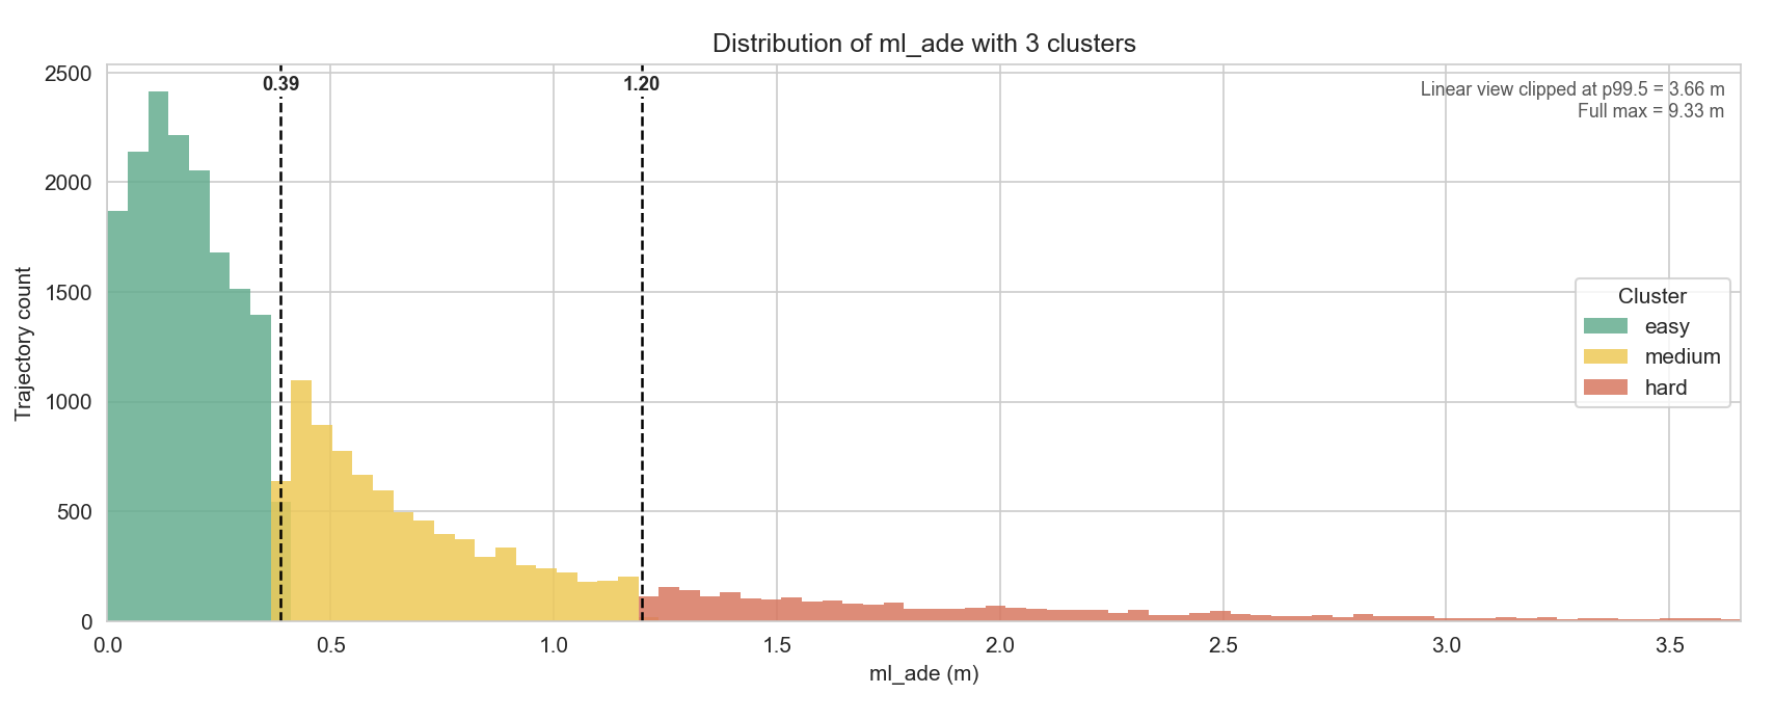
\includegraphics[width=\linewidth]{figures/performance_groups.png}
    \caption{Distribution of \texttt{ml\_ade} with the k-means performance groups. The vertical dashed lines mark the easy/medium and medium/hard boundaries on the original ADE scale.}
    \label{fig:performance_groups}
  \end{minipage}
  \hfill
  \begin{minipage}[t]{0.40\textwidth}
    \centering
    \vspace{0pt}
    {\small
    \captionof{table}{Performance groups from k-means on $\log(1+\texttt{ml\_ade})$.}
    \label{tab:performance_groups}}
    
    \footnotesize
    \renewcommand{\arraystretch}{1.12}
    {\setlength{\tabcolsep}{3pt}
    \begin{tabular}{@{}lccc@{}}
      \toprule
      \textbf{Group} & \textbf{Range} & \textbf{N} & \textbf{Share} \\
      \midrule
      Easy   & $<0.39$ m       & 15,823 & 59\% \\
      Medium & $0.39$--$1.20$ m & 8,320  & 31\% \\
      Hard   & $>1.20$ m       & 2,743  & 10\% \\
      \midrule
      Total  &                  & 26,886 & 100\% \\
      \bottomrule
    \end{tabular}
    }
  \end{minipage}
\end{figure}

The split preserves the main structure of the target distribution: most trajectories are low-error cases, while a smaller hard group captures the heavy right tail. The maximum observed \texttt{ml\_ade} in this analysis is $9.33$ m, substantially above the hard-group threshold.

Second, within each performance group we cluster the signed feature-effect vectors rather than the raw trajectory features directly. Formally, for trajectory $i$ we define one four-dimensional effect vector per meta-model. For the XGBoost meta-model, the vector consists of the SHAP contributions for \texttt{std\_speed}, \texttt{max\_speed}, \texttt{heading\_change\_per\_sec}, and \texttt{mean\_acceleration}. For the GAM, the analogous vector consists of the corresponding additive smooth contributions:

\begin{equation}
  \mathbf{v}^{\mathrm{XGB}}_i =
  \left(\phi_{i,1}, \ldots, \phi_{i,4}\right),
  \qquad
  \mathbf{v}^{\mathrm{GAM}}_i =
  \left(s_1(x_{i,1}), \ldots, s_4(x_{i,4})\right),
  \label{eq:cluster_effect_vectors}
\end{equation}

where the four dimensions correspond to the main MI\,+\,VIF motion features: speed variability, maximum speed, heading change per second, and mean acceleration. Clustering in this effect space groups trajectories by the explanation pattern assigned by the meta-model: two trajectories are close if the same features push their predicted ADE up or down in a similar way.

We compared OPTICS and HDBSCAN within each performance group and selected candidates using three criteria: Density-Based Clustering Validation (DBCV), the share of points labelled as noise, and semantic quality after mapping the clusters back to the raw trajectory characteristics. DBCV is an internal score for density-based cluster structure with range $[-1,1]$; values near $+1$ indicate well-separated dense groups, while values near $0$ indicate ambiguous density structure. Appendix~\ref{app:dbcv_details} gives the formal definition used to read this score.

\begin{table}[H]
  \centering
  
  \caption{Primary XGBoost effect-space clustering selection. OPTICS is compared with the best HDBSCAN candidate for the same performance group.}
  \label{tab:cluster_selection}
  \small
  \renewcommand{\arraystretch}{1.12}
  \begin{tabular}{lcccccc}
    \toprule
    & \multicolumn{3}{c}{\textbf{Selected OPTICS}} & \multicolumn{3}{c}{\textbf{Best HDBSCAN}} \\
    \cmidrule(lr){2-4}\cmidrule(l){5-7}
    \textbf{Group} & \textbf{K} & \textbf{Noise} & \textbf{DBCV} & \textbf{K} & \textbf{Noise} & \textbf{DBCV} \\
    \midrule
    Easy   & 2 & 30\% & 0.41 & 3 & 30\% & 0.30 \\
    Medium & 2 & 40\% & 0.40 & 3 & 24\% & 0.04 \\
    Hard   & 4 & 75\% & 0.09 & 4 & 73\% & 0.05 \\
    \bottomrule
  \end{tabular}
\end{table}

Overall, the primary regime analysis uses OPTICS on XGBoost SHAP effect vectors. In the XGBoost effect space, OPTICS achieved higher DBCV than HDBSCAN for every performance group and produced the clearest easy and medium structures. The choice of XGBoost as the primary effect source is also supported by the model-selection results in Table~\ref{tab:model_variant_selection}: XGBoost fits the per-trajectory loss better than the GAM, and its selected effect-space clusters were semantically clearer after mapping them back to raw motion characteristics. The GAM additive-effect clustering was retained as a robustness check: it showed comparable easy-regime structure and corroborated the hard-regime speed-variation and turning pattern, but it produced weaker medium separation. Figure~\ref{fig:xgboost_optics_umaps} shows the selected XGBoost--OPTICS UMAP diagnostics with noise retained and removed. Appendix Table~\ref{tab:appendix_cluster_candidates} reports the corresponding OPTICS and HDBSCAN candidate scores for both XGBoost and GAM, and Appendix~\ref{app:cluster_umaps} shows the analogous UMAP diagnostics for the remaining algorithm--model combinations. The low hard-regime DBCV and high noise share in Table~\ref{tab:cluster_selection} are important caveats: the hard cases contain weaker, noisier density structure than the easy and medium cases.

\begin{figure}[H]
  \centering
  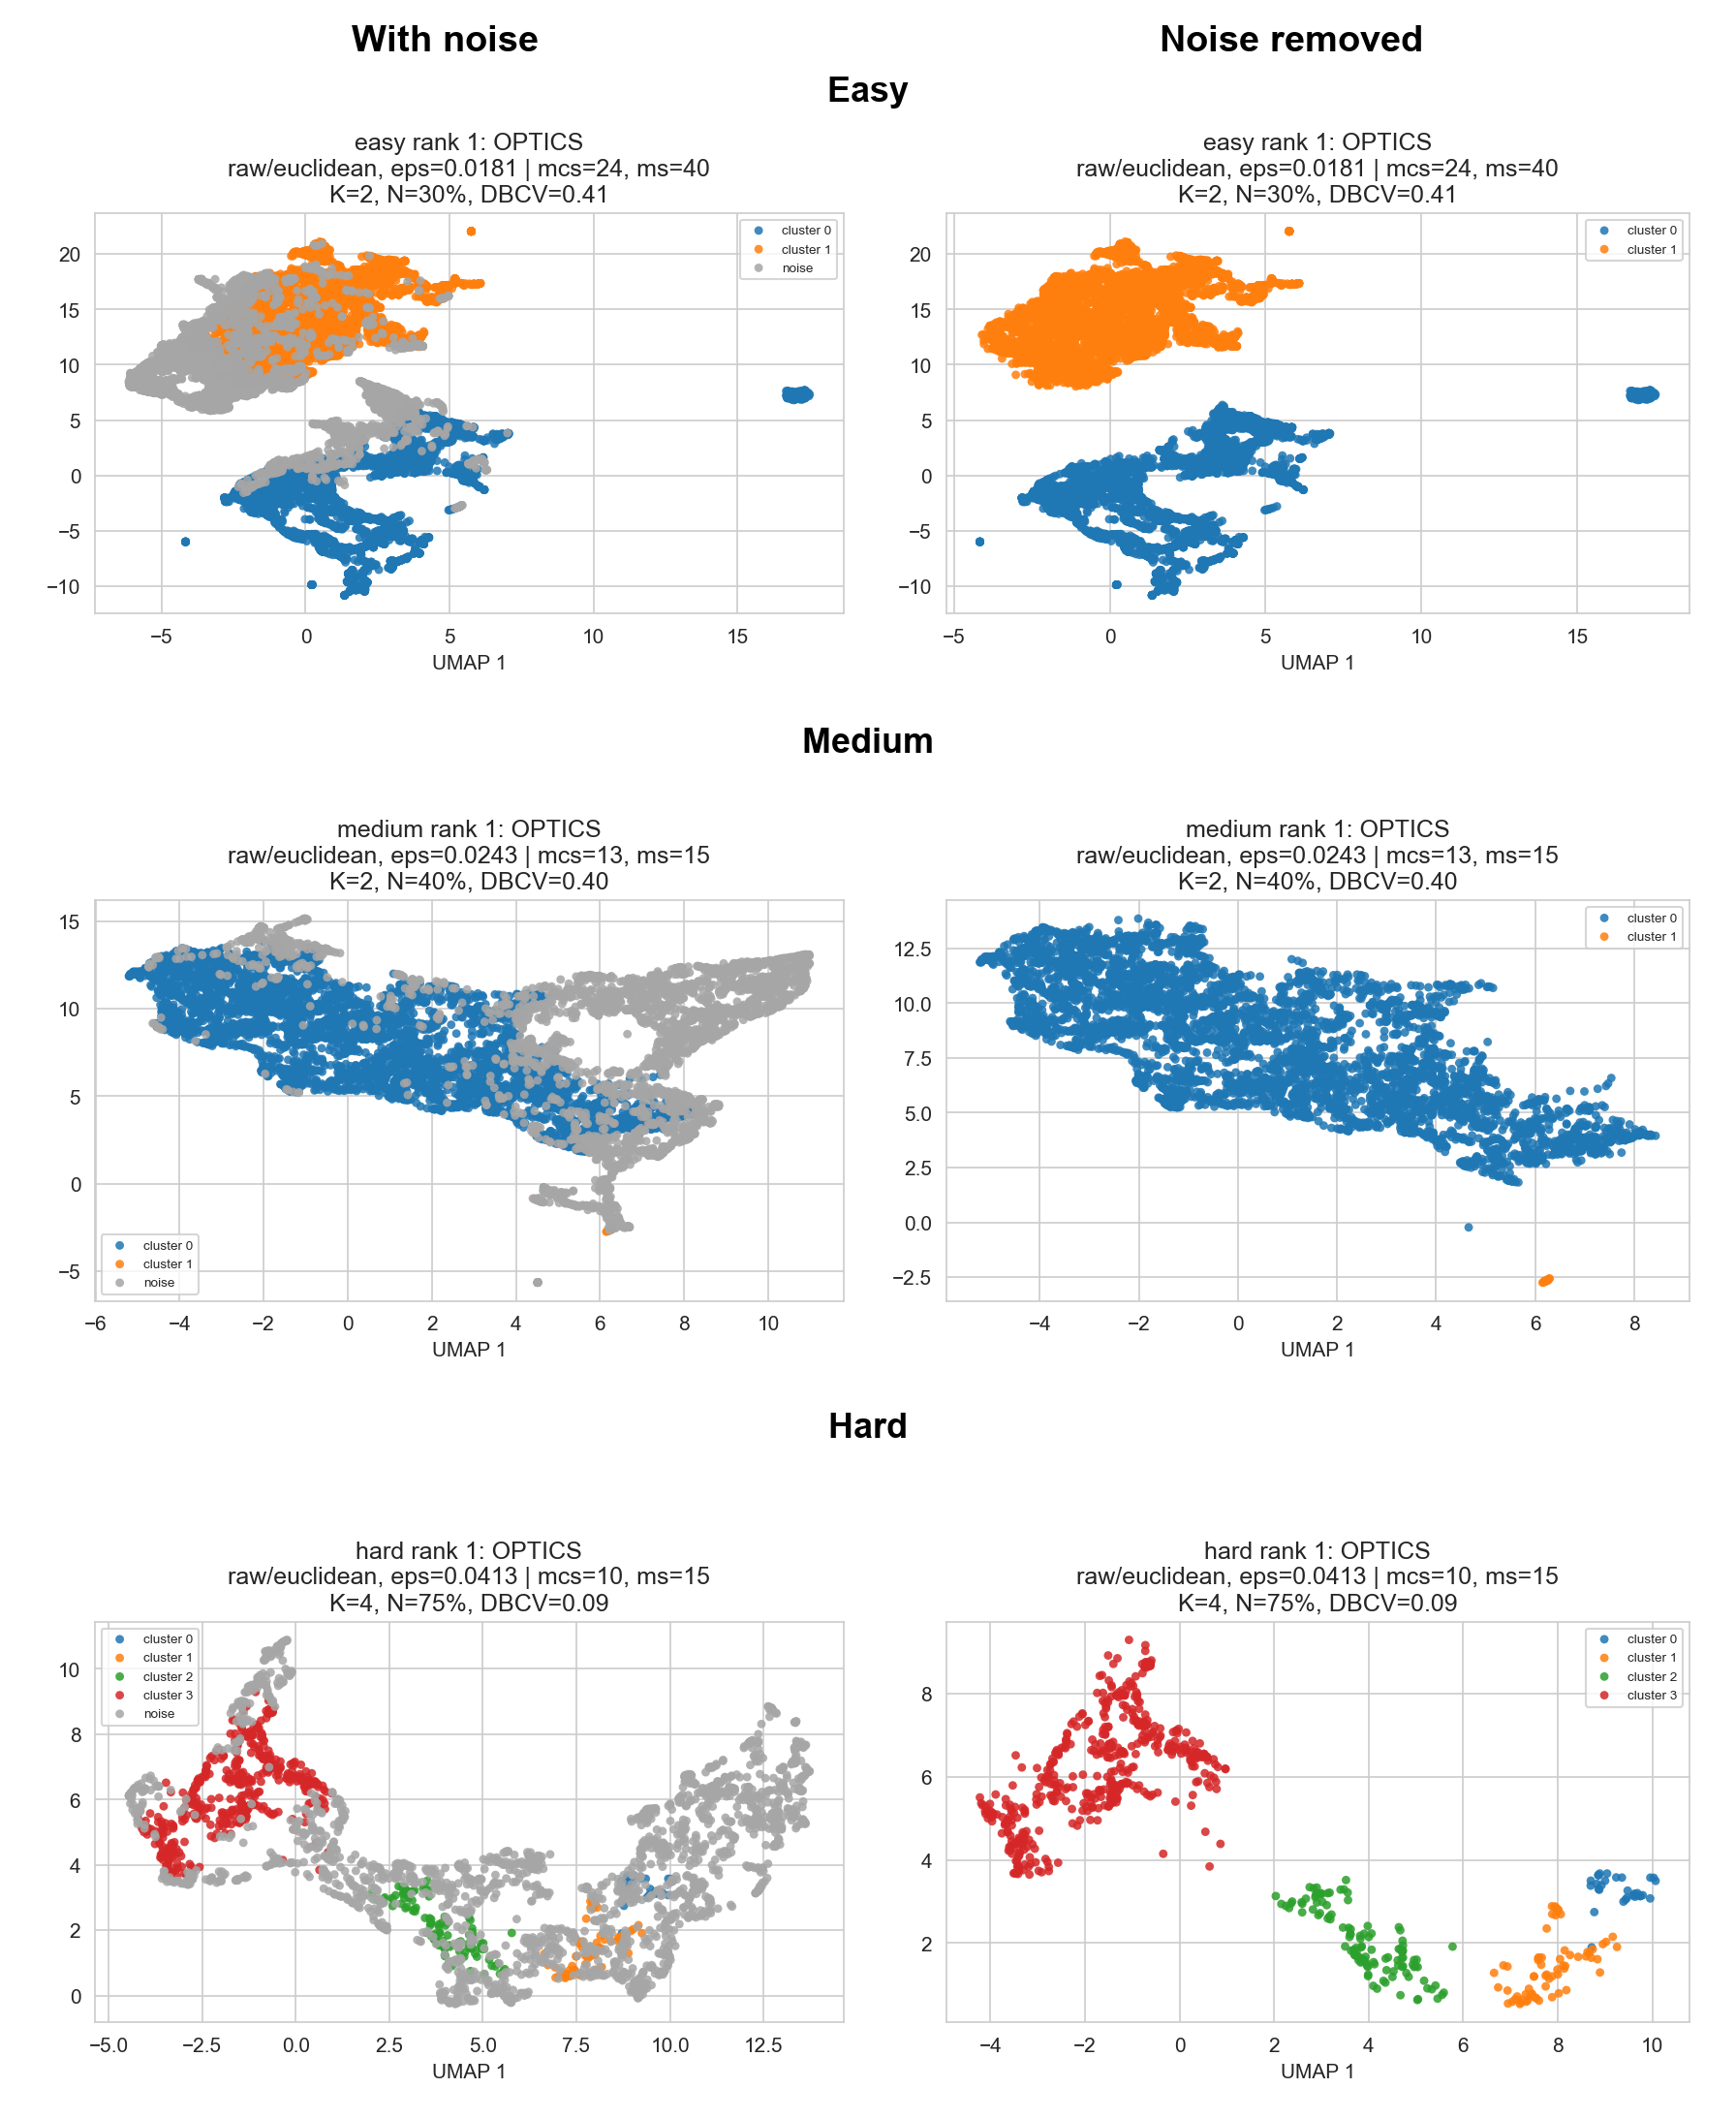
\includegraphics[width=0.86\textwidth]{figures/cluster_umap_xgboost_optics_noise_compare.png}
  \caption{Selected XGBoost--OPTICS effect-space UMAP diagnostics. Rows show the easy, medium, and hard performance groups; the left column includes OPTICS noise points and the right column removes them. These UMAP projections visualise the four-dimensional SHAP effect vectors from Equation~\ref{eq:cluster_effect_vectors} and were not used as clustering input.}
  \label{fig:xgboost_optics_umaps}
\end{figure}

\subsection{Model Setting Sweep}
\label{sec:settings_sweep}

The analysis described so far holds the Trajectron++ configuration fixed and studies how trajectory and scene characteristics relate to prediction error. RQ3 turns to a complementary question: how does the model's own configuration affect prediction quality? To answer this, we conducted a controlled sweep over three of Trajectron++'s key settings and analysed their effect using the same interpretable meta-modelling framework developed in Section~\ref{sec:interpretable_models}.

\subsection{Sweep Design}

We swept over three model settings:
\begin{itemize}
  \item \texttt{history\_sec} — the length of the observed history window, that is, how much of each agent's past motion the model is given as input.
  \item \texttt{prediction\_sec} — the prediction horizon, that is, how far into the future the model forecasts.
  \item \texttt{attention\_radius\_m} — the attention radius, the distance in metres within which neighbouring agents are included in the model's interaction graph; agents beyond this radius are excluded from the focal agent's neighbourhood.
\end{itemize}

We performed a Cartesian sweep over these three parameters, evaluating the model at every combination of the swept values. The sweep was carried out on the nuScenes mini split rather than the full dataset, because the repeated retraining and evaluation required by a full Cartesian sweep is computationally prohibitive on the complete dataset. The mini split nonetheless provides sufficient data to detect the principal effects of each setting.

\subsection{Pooled Model and Confound Control}

To isolate the effect of the model settings from the intrinsic difficulty of individual trajectories, we fit a single \emph{pooled} meta-model that includes both the model-setting variables and the trajectory and scene features as predictors. The trajectory and scene features act as control variables: by accounting for the fact that different trajectories are inherently more or less difficult, the pooled model attributes the residual variation in error to the settings themselves. This design allows the effect of, say, the prediction horizon to be estimated while holding trajectory difficulty constant.

A subtle but important issue in this setup is mechanical confounding between the settings and certain trajectory features. Some features scale trivially with a setting: for instance, the total path length of a trajectory grows mechanically with the prediction horizon, simply because a longer horizon covers more time, irrespective of any change in the agent's behaviour or the difficulty of the prediction. If left uncorrected, such features would absorb part of the genuine effect of the setting and distort the analysis. To prevent this, we used setting-agnostic, normalised versions of the affected features, for example \texttt{mean\_path\_length\_per\_second} in place of the raw \texttt{path\_length}. This normalisation ensures that the estimated effects of the model settings reflect genuine changes in prediction difficulty rather than arithmetic artefacts of the sweep.

\section{Results}

\subsection{Feature Effects on Prediction Error}
\label{sec:rq1_results}

Table~\ref{tab:feature_effect_importance} reports the global feature-importance comparison for the two feature sets introduced in Section~\ref{sec:feature_selection}. The values are mean absolute SHAP contributions from the XGBoost meta-model on the log-transformed target scale. The same table also reports whether the corresponding GAM smooth was statistically significant.

\begin{table}[t]
  \centering
  \caption{Global feature importance for the MI\,+\,VIF and VIF-only feature sets. SHAP values are mean absolute XGBoost contributions on the log-target scale; GAM significance is taken from the corresponding GAM fit.}
  \label{tab:feature_effect_importance}
  \small
  \renewcommand{\arraystretch}{1.12}
  \begin{tabular}{@{}lccc@{}}
    \toprule
    \textbf{Feature} & \textbf{MI\,+\,VIF} & \textbf{VIF-only} & \textbf{GAM} \\
    & $|\mathrm{SHAP}|$ & $|\mathrm{SHAP}|$ & \textbf{significance} \\
    \midrule
    \texttt{std\_speed}                & \textbf{0.109} & \textbf{0.129} & yes, both \\
    \texttt{max\_speed}                & 0.103          & --             & yes, MI\,+\,VIF \\
    \texttt{heading\_change\_per\_sec} & 0.090          & 0.070          & yes, both \\
    \texttt{mean\_acceleration}        & 0.026          & 0.027          & yes, both \\
    \midrule
    \texttt{min\_neighbor\_distance}   & --             & 0.027          & yes, VIF-only \\
    \texttt{scene\_density\_VEHICLE}   & --             & 0.020          & no ($p=0.796$) \\
    \texttt{scene\_num\_VEHICLE}       & --             & 0.016          & yes, VIF-only \\
    \bottomrule
  \end{tabular}
\end{table}

The ranking gives a clear answer to RQ1: motion features dominate the explanation of per-trajectory prediction error. In the main MI\,+\,VIF feature set, the three largest XGBoost effects are \texttt{std\_speed} ($0.109$), \texttt{max\_speed} ($0.103$), and \texttt{heading\_change\_per\_sec} ($0.090$). Mean acceleration is much smaller at $0.026$. The VIF-only comparison preserves this ordering in substance: \texttt{std\_speed} remains the largest feature by a clear margin, \texttt{heading\_change\_per\_sec} remains the next important motion feature, and the retained scene or social features have small SHAP magnitudes. In the GAM comparison, all listed terms except \texttt{scene\_density\_VEHICLE} are significant at the $5\%$ level; the non-significant density smooth reinforces that the scene-density signal is weak and unstable.

Figures~\ref{fig:feature_effects_motion} and~\ref{fig:feature_effects_scene_social} show the feature-effect shapes behind this ranking. The XGBoost PDPs are plotted over the feature interval between the 5th and 95th percentiles, while the GAM smooths cover the full observed range. The two plots should therefore be read together: the PDP gives the black-box model's average effect in the data-dense range, and the GAM smooth checks whether an additive model recovers a compatible marginal pattern.

\begin{figure}[t]
  \centering
  \begin{minipage}{0.49\textwidth}
    \centering
    \textbf{\texttt{std\_speed}}\\[0.2em]
    \begin{minipage}{0.48\linewidth}
      \centering
      \scriptsize XGBoost PDP\\[0.1em]
      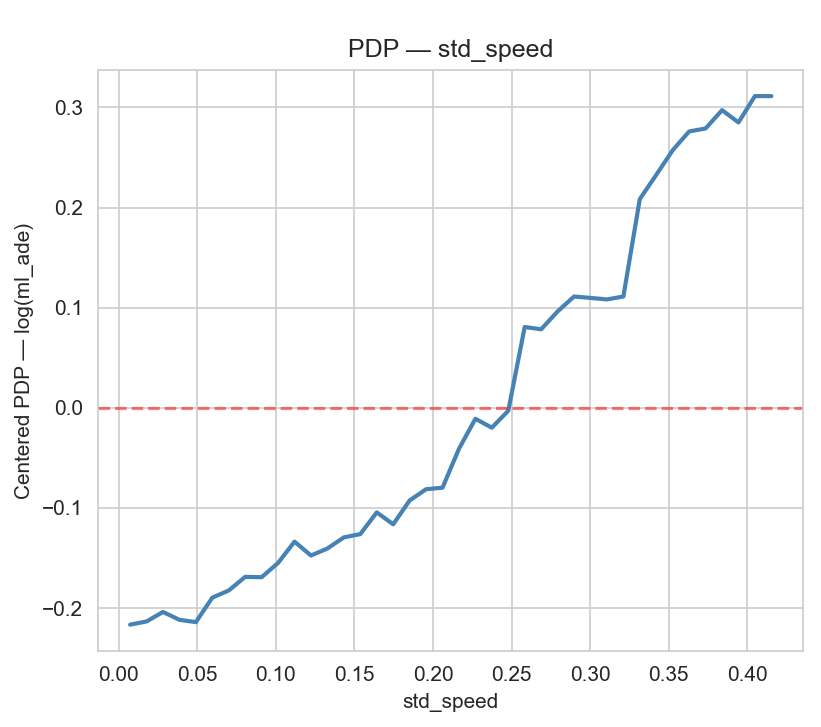
\includegraphics[width=\linewidth]{figures/pdp_std_speed.png}
    \end{minipage}
    \hfill
    \begin{minipage}{0.48\linewidth}
      \centering
      \scriptsize GAM smooth\\[0.1em]
      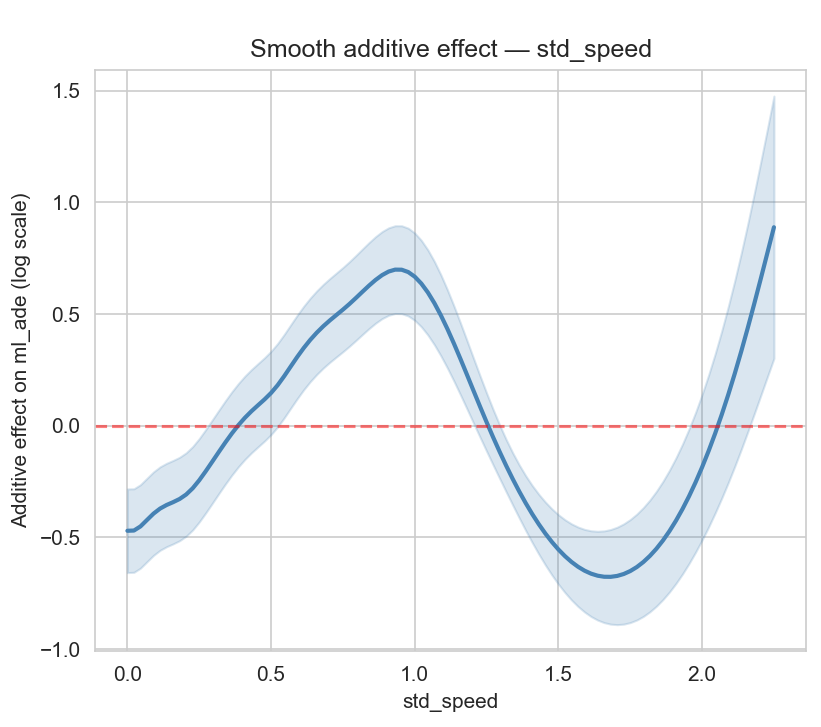
\includegraphics[width=\linewidth]{figures/gam_std_speed.png}
    \end{minipage}
  \end{minipage}
  \hfill
  \begin{minipage}{0.49\textwidth}
    \centering
    \textbf{\texttt{heading\_change\_per\_sec}}\\[0.2em]
    \begin{minipage}{0.48\linewidth}
      \centering
      \scriptsize XGBoost PDP\\[0.1em]
      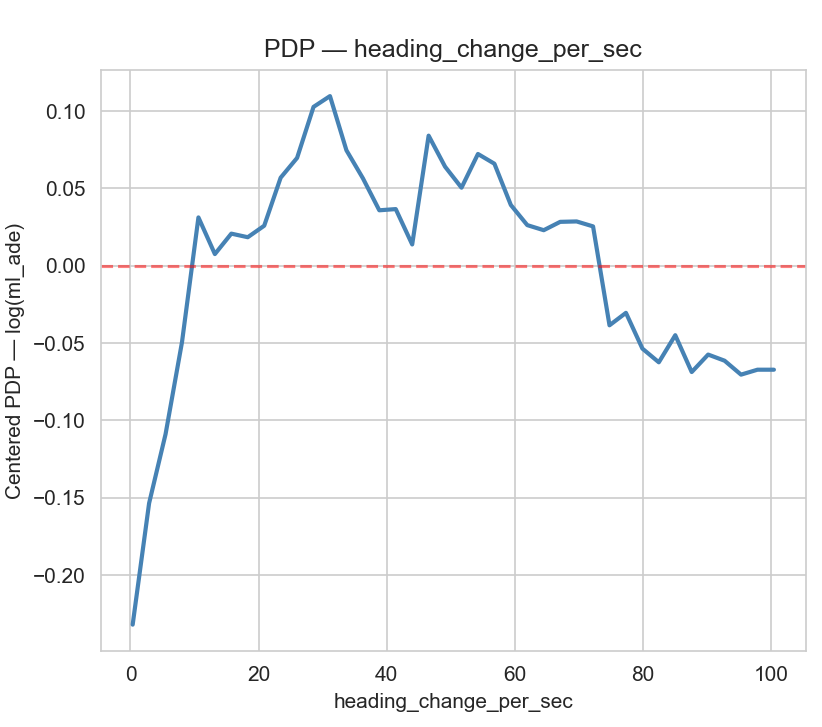
\includegraphics[width=\linewidth]{figures/pdp_heading_change_per_sec.png}
    \end{minipage}
    \hfill
    \begin{minipage}{0.48\linewidth}
      \centering
      \scriptsize GAM smooth\\[0.1em]
      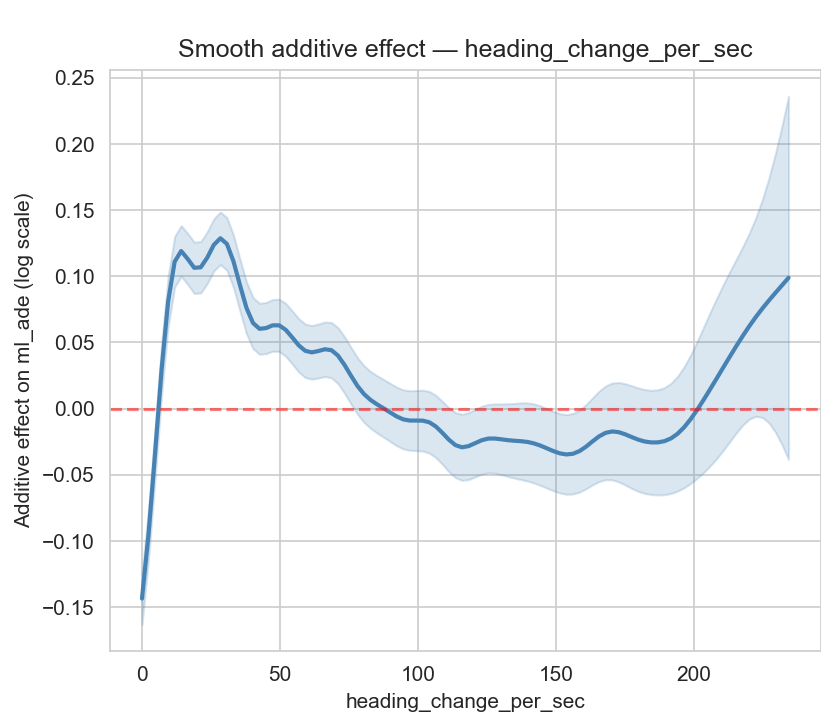
\includegraphics[width=\linewidth]{figures/gam_heading_change_per_sec.png}
    \end{minipage}
  \end{minipage}

  \vspace{0.7em}

  \begin{minipage}{0.49\textwidth}
    \centering
    \textbf{\texttt{max\_speed}}\\[0.2em]
    \begin{minipage}{0.48\linewidth}
      \centering
      \scriptsize XGBoost PDP\\[0.1em]
      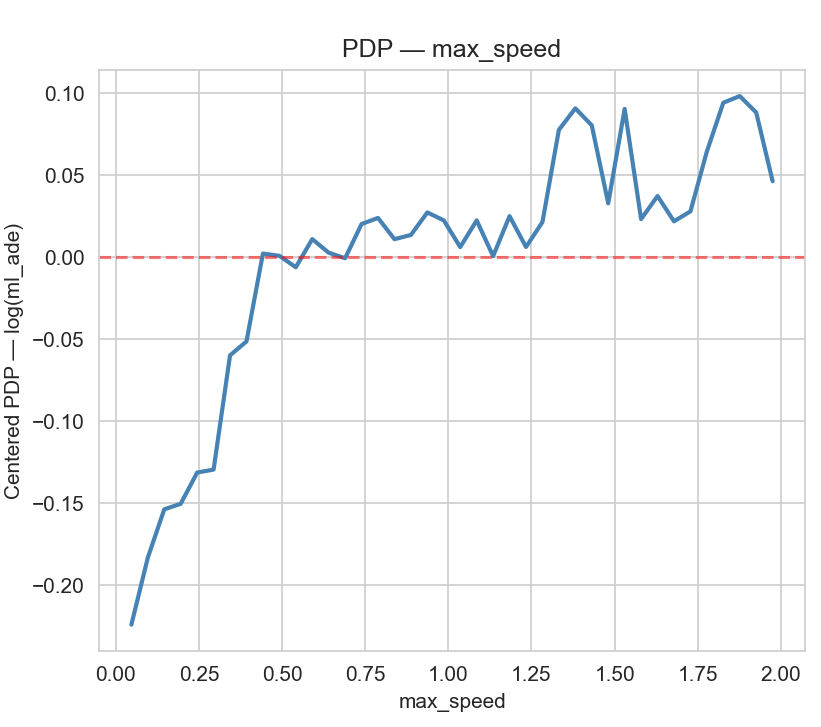
\includegraphics[width=\linewidth]{figures/pdp_max_speed.png}
    \end{minipage}
    \hfill
    \begin{minipage}{0.48\linewidth}
      \centering
      \scriptsize GAM smooth\\[0.1em]
      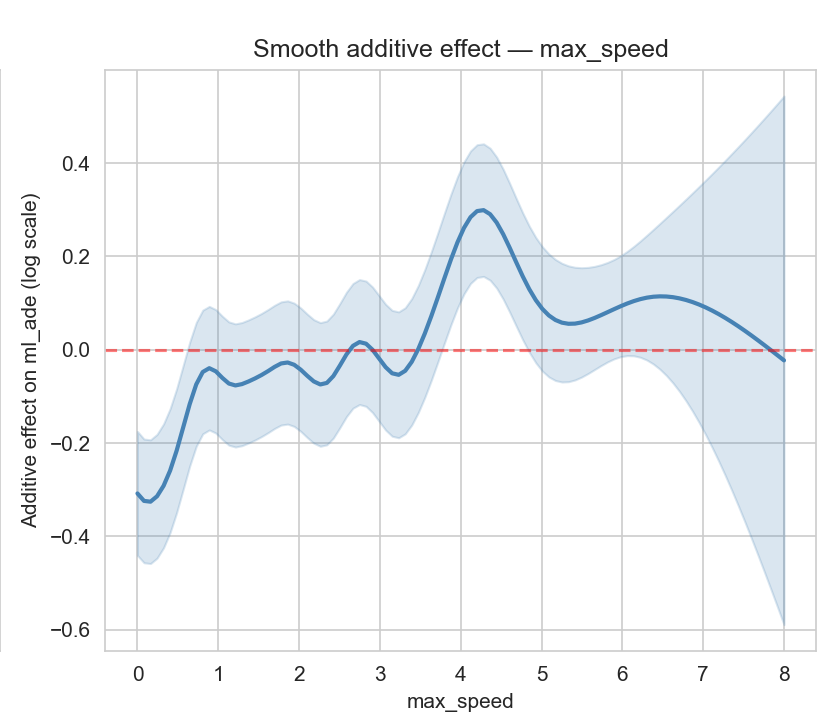
\includegraphics[width=\linewidth]{figures/gam_max_speed.png}
    \end{minipage}
  \end{minipage}
  \hfill
  \begin{minipage}{0.49\textwidth}
    \centering
    \textbf{\texttt{mean\_acceleration}}\\[0.2em]
    \begin{minipage}{0.48\linewidth}
      \centering
      \scriptsize XGBoost PDP\\[0.1em]
      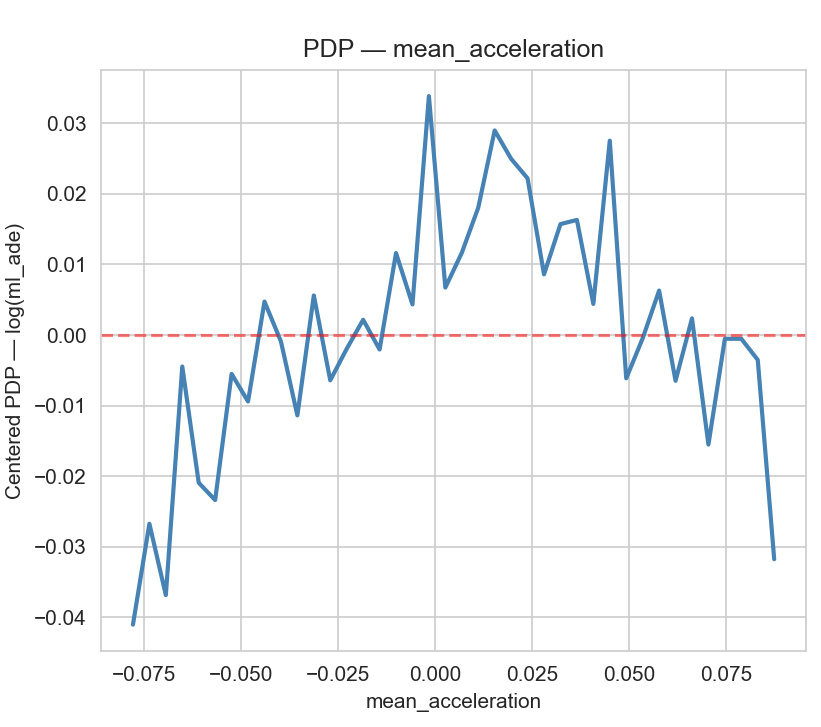
\includegraphics[width=\linewidth]{figures/pdp_mean_acceleration.png}
    \end{minipage}
    \hfill
    \begin{minipage}{0.48\linewidth}
      \centering
      \scriptsize GAM smooth\\[0.1em]
      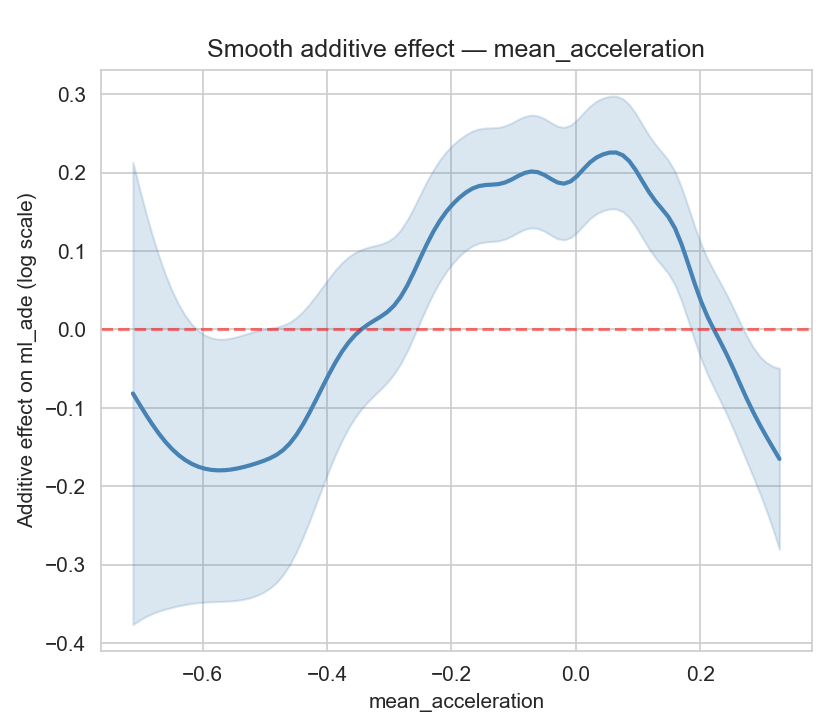
\includegraphics[width=\linewidth]{figures/gam_mean_acceleration.png}
    \end{minipage}
  \end{minipage}
  \caption{Feature-effect plots for the four motion features retained in the main MI\,+\,VIF feature set.}
  \label{fig:feature_effects_motion}
\end{figure}

The strongest and most stable effect is \texttt{std\_speed}. Its XGBoost PDP increases monotonically across the feature interval shown in the PDP, and over that same interval, the GAM smooth supports the positive trend observed in the PDP. Trajectories whose speed varies more strongly therefore receive larger predicted ADE: erratic speed is harder for Trajectron++ to forecast. \texttt{heading\_change\_per\_sec} is also important but less monotone. Both models show that turning raises error in the low-to-moderate range, while the effect flattens or drops at high heading-change values where the relationship is less stable.

\texttt{max\_speed} is the third major motion feature. The XGBoost PDP is broadly increasing, and the GAM smooth agrees over the feature interval shown in the PDP, although its confidence interval widens in the high-speed tail. Peak speed therefore contributes to error, but it is weaker than speed variability and turning. By contrast, \texttt{mean\_acceleration} has a small global SHAP value and a mixed effect shape. Its PDP oscillates around zero and the GAM smooth is not as stable as the leading motion features. This means that acceleration is detectable in the additive significance test, but its population-level effect is small compared with the dominant speed-variation and heading-change effects. A useful interpretation is that prediction error is driven more by how often a pedestrian changes speed than by the presence of non-zero acceleration alone.

The scene-context comparison is weaker. \texttt{scene\_density\_VEHICLE} has only a small VIF-only SHAP value ($0.020$), a noisy PDP, and a non-significant GAM smooth. The other retained VIF-only scene or social features are also small: \texttt{scene\_num\_VEHICLE} has mean absolute SHAP $0.016$, and \texttt{min\_neighbor\_distance} has $0.027$. Both are significant in the VIF-only GAM, so they are not pure noise, but their SHAP magnitudes remain small enough to support the broader conclusion that scene and social features are secondary. The main message is therefore not that scene context is irrelevant in principle, but that these engineered scene and social descriptors do not robustly explain individual Trajectron++ error in this analysis. Within the current feature representation, the focal agent's own motion dominates.

\newpage
\begin{figure}[t]
  \centering
  \begin{minipage}{0.49\textwidth}
    \centering
    \textbf{\texttt{scene\_num\_VEHICLE}}\\[0.2em]
    \begin{minipage}{0.48\linewidth}
      \centering
      \scriptsize XGBoost PDP\\[0.1em]
      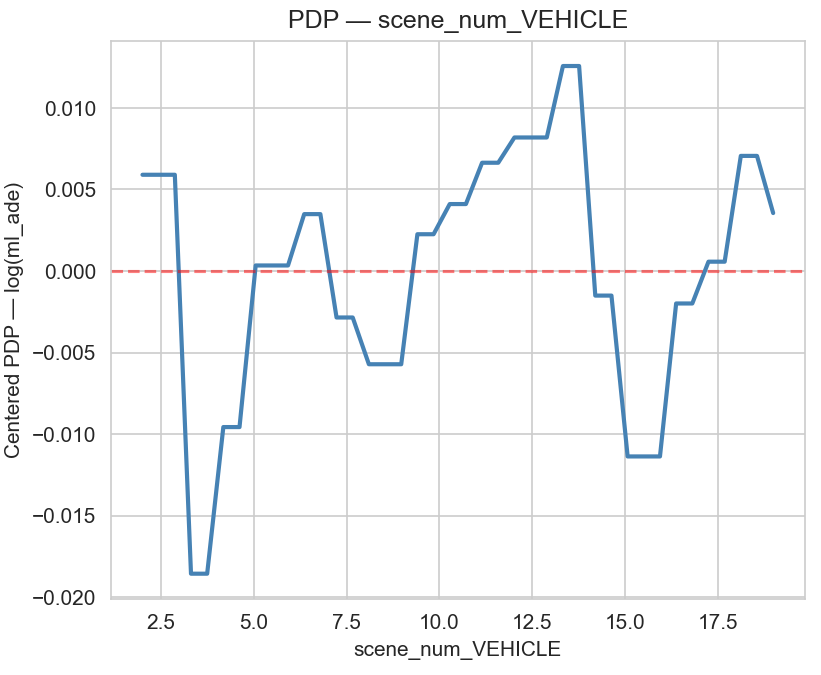
\includegraphics[width=\linewidth]{figures/pdp_scene_num_vehicle.png}
    \end{minipage}
    \hfill
    \begin{minipage}{0.48\linewidth}
      \centering
      \scriptsize GAM smooth\\[0.1em]
      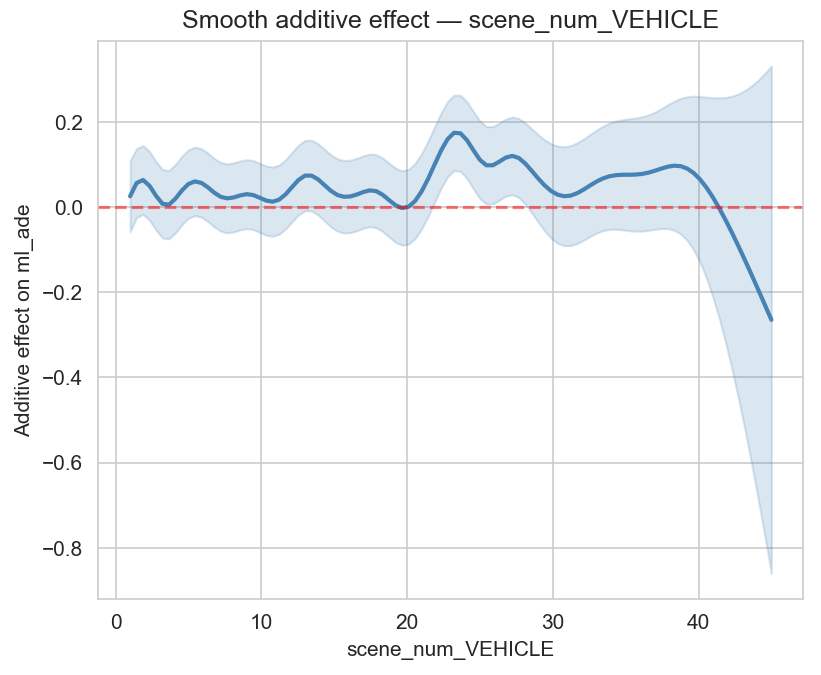
\includegraphics[width=\linewidth]{figures/gam_scene_num_vehicle.png}
    \end{minipage}
  \end{minipage}
  \hfill
  \begin{minipage}{0.49\textwidth}
    \centering
    \textbf{\texttt{scene\_density\_VEHICLE}}\\[0.2em]
    \begin{minipage}{0.48\linewidth}
      \centering
      \scriptsize XGBoost PDP\\[0.1em]
      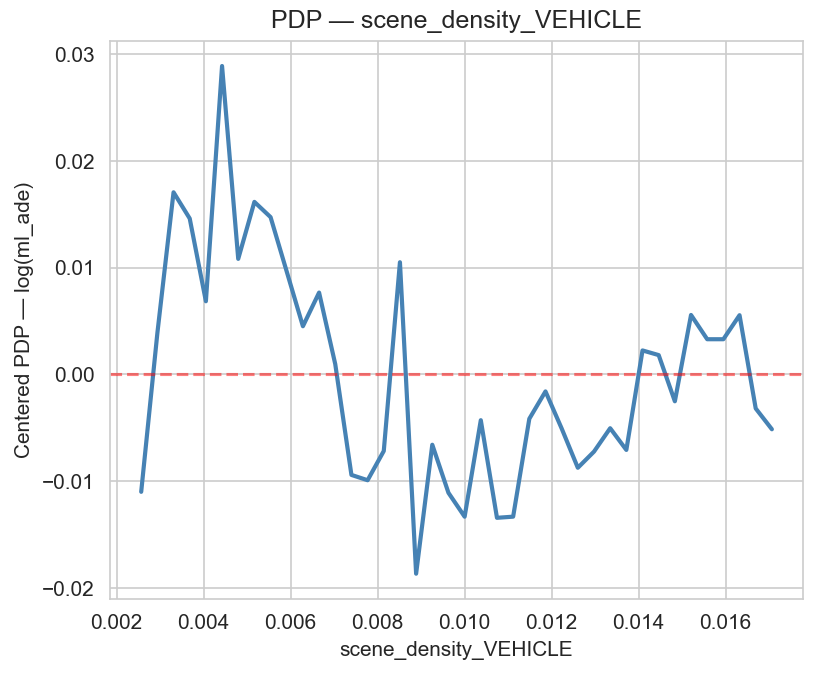
\includegraphics[width=\linewidth]{figures/pdp_scene_density_vehicle.png}
    \end{minipage}
    \hfill
    \begin{minipage}{0.48\linewidth}
      \centering
      \scriptsize GAM smooth\\[0.1em]
      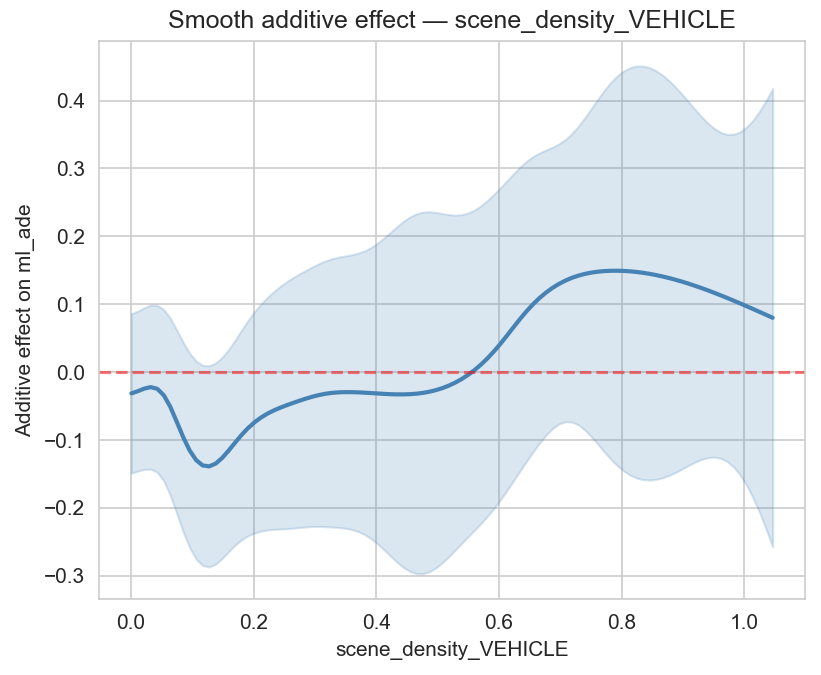
\includegraphics[width=\linewidth]{figures/gam_scene_density_vehicle.png}
    \end{minipage}
  \end{minipage}

  \vspace{0.7em}

  \begin{minipage}{0.49\textwidth}
    \centering
    \textbf{\texttt{min\_neighbor\_distance}}\\[0.2em]
    \begin{minipage}{0.48\linewidth}
      \centering
      \scriptsize XGBoost PDP\\[0.1em]
      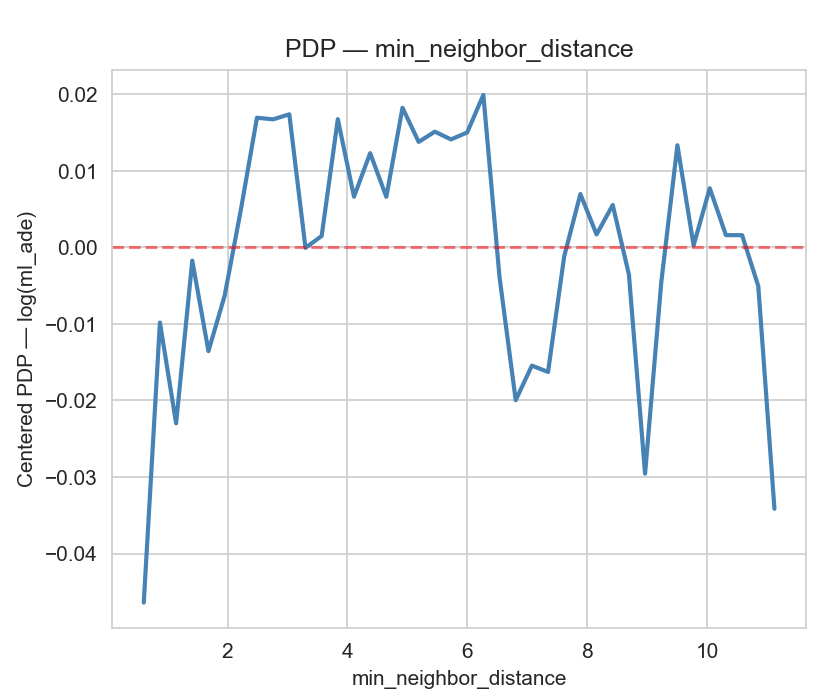
\includegraphics[width=\linewidth]{figures/pdp_min_neighbor_distance.png}
    \end{minipage}
    \hfill
    \begin{minipage}{0.48\linewidth}
      \centering
      \scriptsize GAM smooth\\[0.1em]
      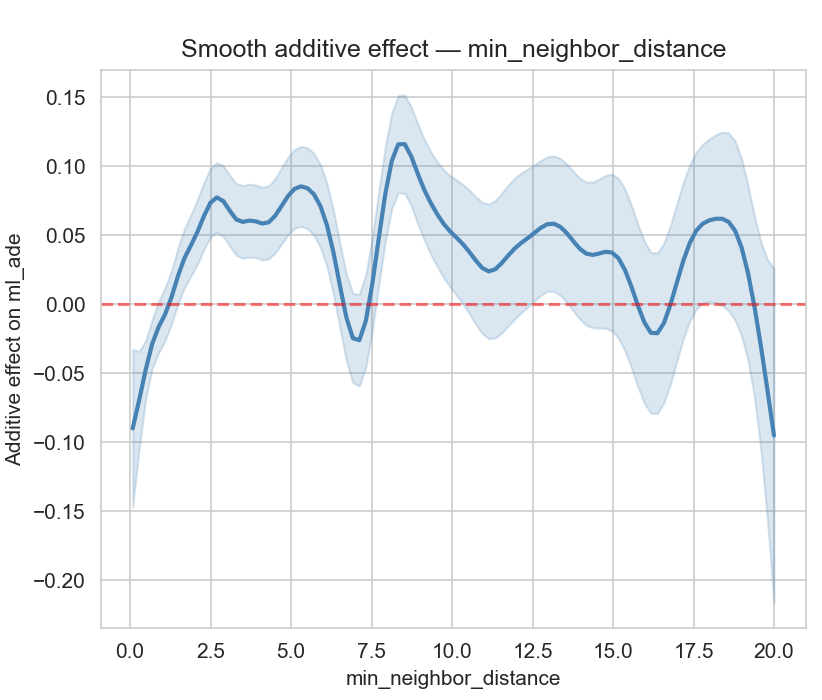
\includegraphics[width=\linewidth]{figures/gam_min_neighbor_distance.png}
    \end{minipage}
  \end{minipage}
  \hfill\null
  \caption{Feature-effect plots for the social and scene-context features retained by the VIF-only feature set.}
  \label{fig:feature_effects_scene_social}
\end{figure}

\subsection{Success and Failure Modes}
\label{sec:rq2_results}

Using the performance grouping and feature-effect clustering defined in Section~\ref{sec:cluster_methodology}, we interpret the selected clusters as explanation patterns for RQ2 rather than as clusters of raw trajectory coordinates.

The feature effects resolve into coherent behavioural regimes. The model succeeds on two broad classes of trajectory: slow turners, where low speed bounds the impact of turning, and straight walkers, where stable heading bounds the impact of speed. Conversely, the failure mode is erratic motion in which speed variability and turning occur together. Crucially, raw speed alone is not a failure driver; high speed becomes problematic only when paired with turning. The hardest cases for Trajectron++ are thus those that combine the two dominant difficulty factors simultaneously.

\newpage
\subsection{Feature Importance of Model Settings}
\label{sec:settings_importance}

Applying the pooled meta-model of Section~\ref{sec:settings_sweep}, we quantified the influence of each model setting on prediction error using mean absolute SHAP values from the XGBoost model, cross-validated against the GAM. Table~\ref{tab:settings_shap} reports the resulting global feature importance.

\begin{table}[h]
  \centering
  \caption{Mean absolute SHAP values from the pooled XGBoost model, ranking the influence of model settings and trajectory features on per-trajectory prediction error. Larger values indicate greater influence.}
  \label{tab:settings_shap}
  \begin{tabular}{l c}
    \toprule
    \textbf{Feature} & \textbf{Mean} $|\text{SHAP}|$ \\
    \midrule
    \texttt{prediction\_sec}        & \textbf{0.178} \\
    \texttt{attention\_radius\_m}   & 0.098 \\
    \texttt{std\_speed}             & 0.093 \\
    \texttt{max\_speed}             & 0.070 \\
    \texttt{heading\_change\_per\_sec} & 0.039 \\
    \texttt{min\_neighbor\_distance}   & 0.029 \\
    \texttt{history\_sec}           & 0.022 \\
    \texttt{mean\_acceleration}     & 0.013 \\
    \bottomrule
  \end{tabular}
\end{table}

The most striking observation is that the two highest-ranked features are model settings rather than trajectory characteristics. The prediction horizon, \texttt{prediction\_sec}, is by a clear margin the most influential feature overall, with a mean absolute SHAP value of $0.178$, and the attention radius, \texttt{attention\_radius\_m}, ranks second at $0.098$. The trajectory features, led by \texttt{std\_speed} at $0.093$, remain significant contributors but are surpassed by these two settings. In other words, within the swept ranges, the choice of configuration influences prediction quality at least as strongly as the intrinsic properties of the trajectories being predicted.

All eight features in the pooled model are also statistically significant in the GAM ($p \ll 0.01$), confirming that the effects are not specific to the tree-based model. The two meta-models do, however, differ markedly in fit quality: XGBoost achieves $R^2 = 0.90$ with an RMSE of $0.13$, substantially better than the GAM's $R^2 = 0.65$ and RMSE of $0.24$. This gap is itself informative. Because the GAM is purely additive while XGBoost can represent interactions, the superior fit of the latter indicates that meaningful interaction effects exist between the model settings and the trajectory features, effects that an additive model cannot capture.

We now examine each setting in turn through its partial dependence plot (PDP), which shows the average direction and shape of its effect on the log-scale prediction error.

\subsection{Prediction Horizon}

The prediction horizon exhibits the largest effect of any feature. Its partial dependence plot rises monotonically: as the horizon lengthens, the prediction error grows. This is intuitively unsurprising, since forecasting further into the future is inherently harder and accumulated uncertainty compounds over time. The value of the analysis lies in quantifying this effect and establishing that, within our experimental range, the horizon setting exerts a stronger influence on prediction quality than any intrinsic trajectory characteristic.

\subsection{Attention Radius}

The attention radius is the second most influential feature, and its effect is more nuanced than that of the horizon. A larger radius admits more neighbouring agents into the focal agent's interaction graph, supplying additional context. One might expect more context to be uniformly beneficial, but the partial dependence plot reveals a non-linear relationship. At very small radii, performance is poor because the model omits genuinely relevant neighbours. Beyond a certain point, however, enlarging the radius begins to introduce distant, irrelevant agents whose inclusion adds noise rather than signal. The plot indicates that a comparatively short attention radius is beneficial in this dataset, with performance degrading as the radius becomes large. This points to the existence of an intermediate optimal range rather than a ``larger-is-better'' rule.

\subsection{History Window}

The history window has the smallest effect of the three settings. Its partial dependence plot is comparatively flat across the swept range, indicating that the model is robust to the amount of past motion it observes, at least within the values we tested. From a practical standpoint, this is a reassuring finding: it suggests that Trajectron++ does not depend critically on a long observation window to produce reasonable predictions, and that the history length can be chosen with relatively little concern for its impact on accuracy within this regime.

\section{Conclusion and Discussion}
\label{sec:conclusion}

This work set out to look beyond aggregate error metrics and ask \emph{why} some trajectories are harder for Trajectron++ to predict than others. By recovering per-trajectory prediction errors, relating them to interpretable trajectory and scene features through GAM and XGBoost meta-models, and conducting a controlled sweep over model settings, we have characterised the model's competence in a fine-grained and actionable way.

The results reveal that trajectory characteristics, particularly speed variability and turning, are dominant drivers of prediction difficulty. Model configuration also plays a critical role, with the prediction horizon and attention radius exerting effects comparable to the trajectory features themselves. These findings provide concrete guidance for understanding and improving trajectory prediction performance.

\subsection{Limitations}

Several limitations should temper the interpretation of these findings. First, our meta-models explain Trajectron++, not ground-truth difficulty. The identified drivers are inferred through the meta-models as proxies, since Trajectron++ does not expose its internal reasoning directly; the effects we report are therefore model-specific and may not generalise to other prediction architectures.

Second, the meta-model under-predicts at high ADE. Out-of-fold diagnostics show strong agreement between predicted and actual error at low-to-moderate ADE but systematic under-prediction in the high-error tail. The implication is that our trajectory and scene features do not fully capture what makes the worst cases worst: factors such as map and lane geometry, location, or finer-grained social context appear to be missing from the current feature set. This shortfall is the most likely reason that the clustering of hard cases is comparatively weak, as the available feature effects do not differentiate cleanly within the high-error tail.

Third, the scope of the study is bounded. We predict pedestrian trajectories on nuScenes only, so there is no guarantee that the conclusions transfer to other agent types or to other datasets. Moreover, the settings sweep was conducted on the nuScenes mini split for reasons of computational cost, and its results may not transfer directly to full-scale training.

\subsection{Future Work}

These limitations suggest several directions for future work. A central strength of our approach is that the pipeline is model- and dataset-agnostic by design: the meta-modelling and feature-effect clustering are decoupled from the prediction model and the dataset, and through the \texttt{trajdata} interface the same pipeline can be ported to other trajectory prediction models and datasets with little additional effort. This makes broad replication straightforward.

A natural next step is to enrich the input space with map and lane geometry, location information, and finer social context. In particular, enabling and evaluating map-based inputs is reserved for future work rather than part of the present experimental setup. Such features directly target the under-prediction ceiling identified in the diagnostics and may unlock cleaner structure in the hard-error regime that the current feature set fails to separate. Finally, extending the analysis to vehicle, cyclist, and motorcyclist trajectories would test whether the same drivers of difficulty, speed variability and turning, govern prediction error across agent types, or whether each agent class exhibits its own characteristic failure modes.



% ------------------------------------------------------------------------------
% APPENDIX -------------------------------------------------------------------
% ------------------------------------------------------------------------------

\newpage

\pagenumbering{Roman}

\setcounter{page}{5} % CHANGE

\appendix


\section{Appendix}

\subsection{Cluster UMAP Diagnostics}
\label{app:cluster_umaps}

Table~\ref{tab:appendix_cluster_candidates} expands the main XGBoost selection table by adding the corresponding GAM additive-effect candidates. The table reports the rank-1 OPTICS and HDBSCAN candidates within each performance group under the same conservative quality screen used in Section~\ref{sec:cluster_methodology}.

\begin{table}[H]
  \centering
  
  \caption{Rank-1 effect-space clustering candidates for XGBoost SHAP and GAM additive effects. Noise is the share of trajectories labelled as noise by the candidate.}
  \label{tab:appendix_cluster_candidates}
  \footnotesize
  \renewcommand{\arraystretch}{1.12}
  \begin{tabular}{llcccccc}
    \toprule
    & & \multicolumn{3}{c}{\textbf{OPTICS}} & \multicolumn{3}{c}{\textbf{HDBSCAN}} \\
    \cmidrule(lr){3-5}\cmidrule(l){6-8}
    \textbf{Model} & \textbf{Group} & \textbf{K} & \textbf{Noise} & \textbf{DBCV} & \textbf{K} & \textbf{Noise} & \textbf{DBCV} \\
    \midrule
    XGBoost & Easy   & 2 & 30\% & 0.41 & 3 & 30\% & 0.30 \\
    XGBoost & Medium & 2 & 40\% & 0.40 & 3 & 24\% & 0.04 \\
    XGBoost & Hard   & 4 & 75\% & 0.09 & 4 & 73\% & 0.05 \\
    GAM     & Easy   & 4 & 32\% & 0.40 & 5 & 25\% & 0.35 \\
    GAM     & Medium & 3 & 15\% & 0.14 & 2 & 73\% & -0.03 \\
    GAM     & Hard   & 4 & 70\% & 0.19 & 2 & 28\% & 0.12 \\
    \bottomrule
  \end{tabular}
\end{table}

Figure~\ref{fig:xgboost_optics_umaps} gives the primary XGBoost--OPTICS diagnostic in the main text. Figures~\ref{fig:appendix_xgboost_hdbscan_umaps}--\ref{fig:appendix_gam_hdbscan_umaps} show the remaining rank-1 algorithm--model combinations. In each appendix figure, the left column includes noise points and the right column removes them, with easy, medium, and hard performance groups arranged from top to bottom. These are diagnostic projections of the four-dimensional effect vectors from Equation~\ref{eq:cluster_effect_vectors}; they were not used as clustering input.

\begin{figure}[H]
  \centering
  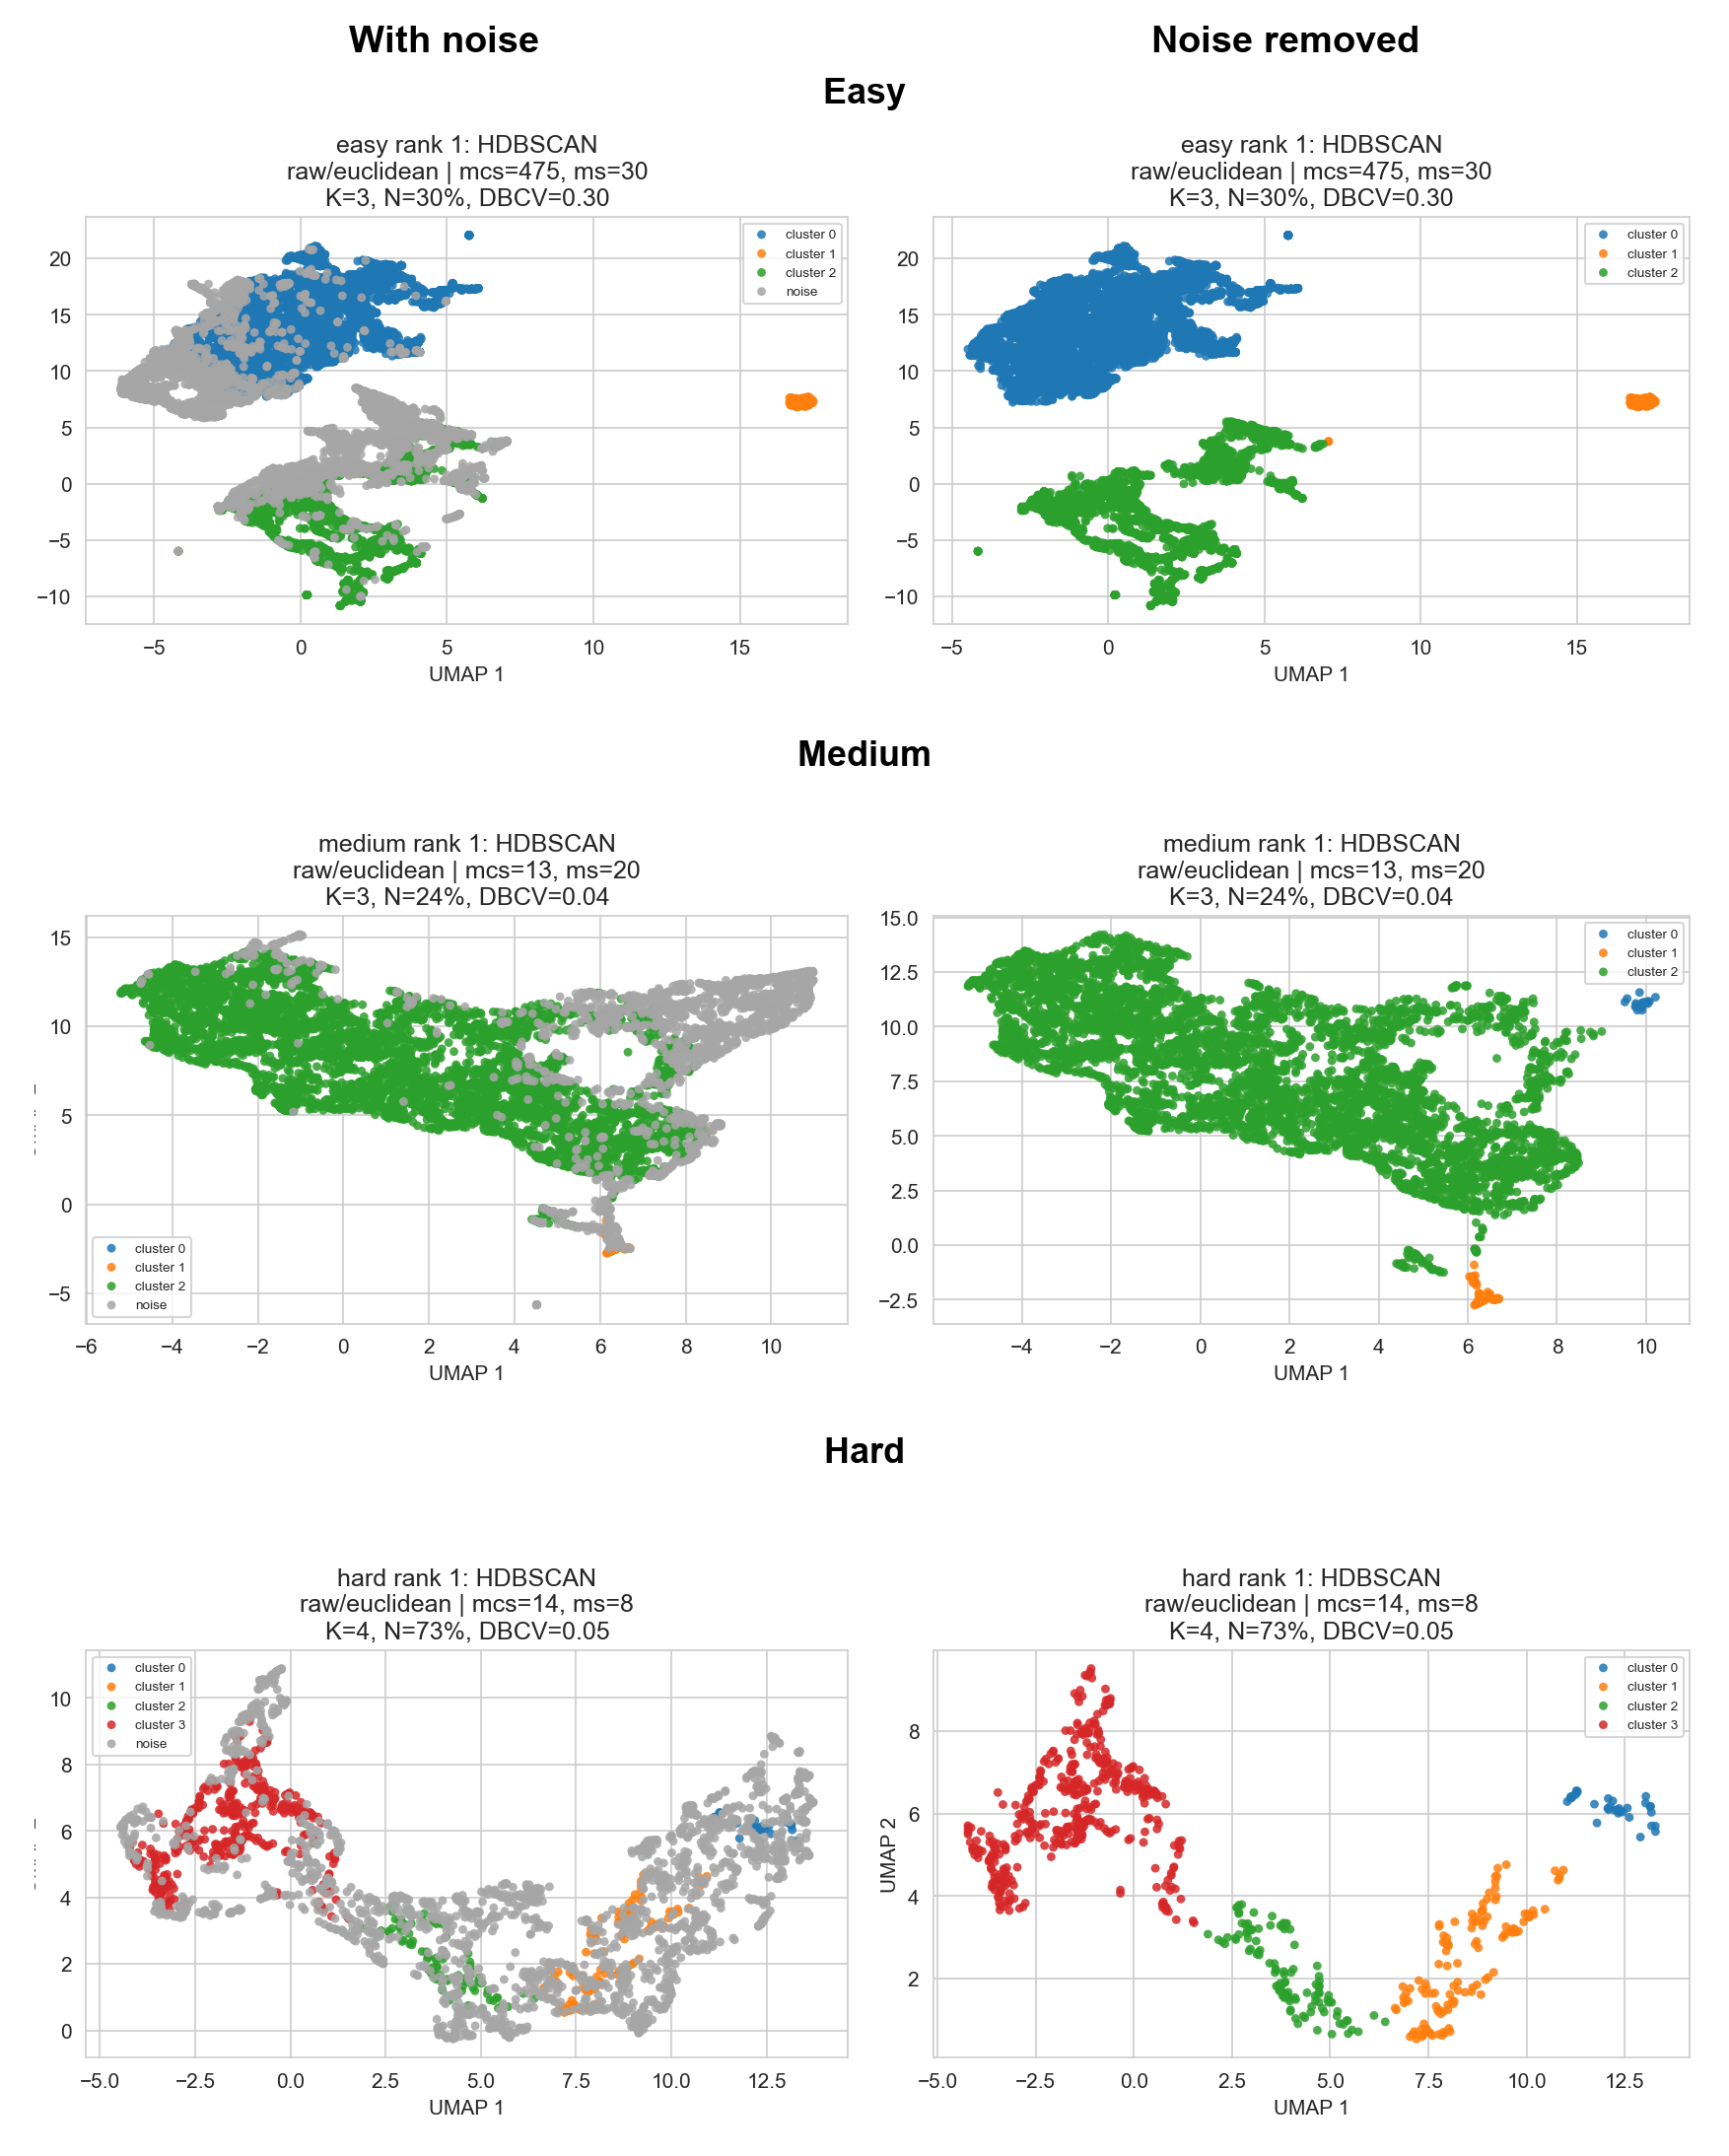
\includegraphics[width=0.86\textwidth]{figures/cluster_umap_xgboost_hdbscan_noise_compare.png}
  \caption{XGBoost--HDBSCAN effect-space UMAP diagnostics. Rows show the easy, medium, and hard performance groups; the left column includes HDBSCAN noise points and the right column removes them.}
  \label{fig:appendix_xgboost_hdbscan_umaps}
\end{figure}

\begin{figure}[H]
  \centering
  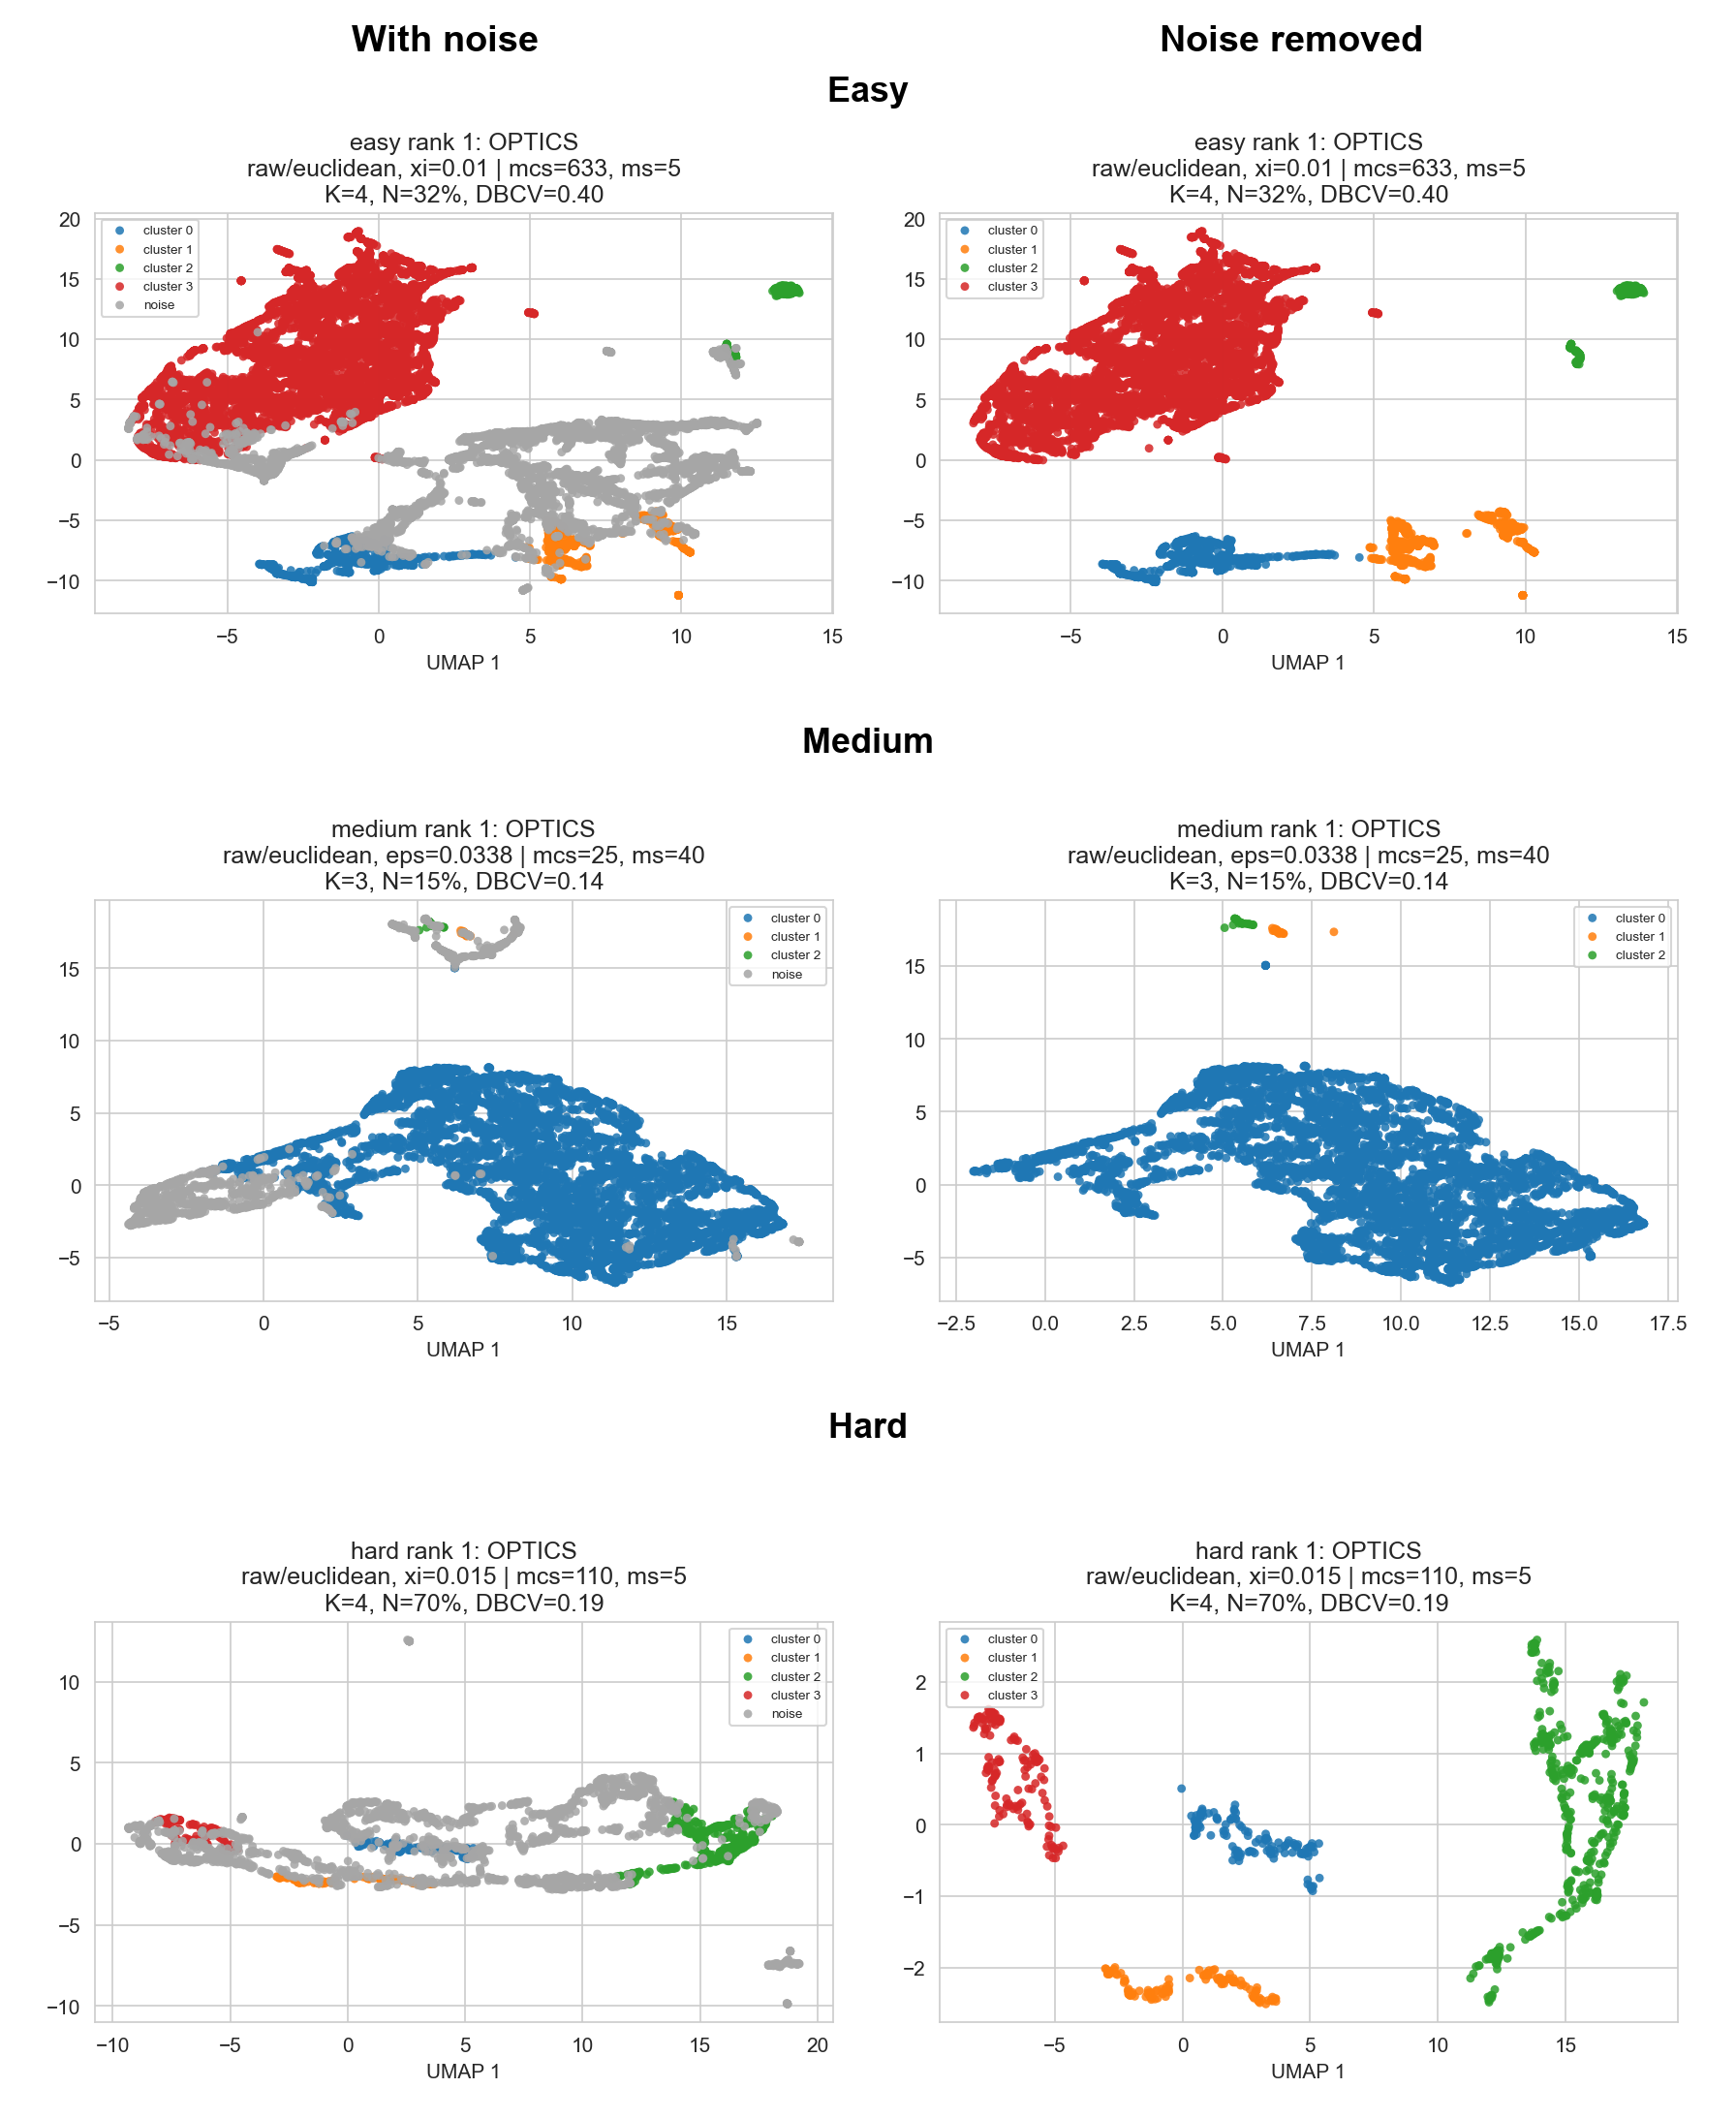
\includegraphics[width=0.86\textwidth]{figures/cluster_umap_gam_optics_noise_compare.png}
  \caption{GAM--OPTICS additive-effect UMAP diagnostics. Rows show the easy, medium, and hard performance groups; the left column includes OPTICS noise points and the right column removes them.}
  \label{fig:appendix_gam_optics_umaps}
\end{figure}

\begin{figure}[H]
  \centering
  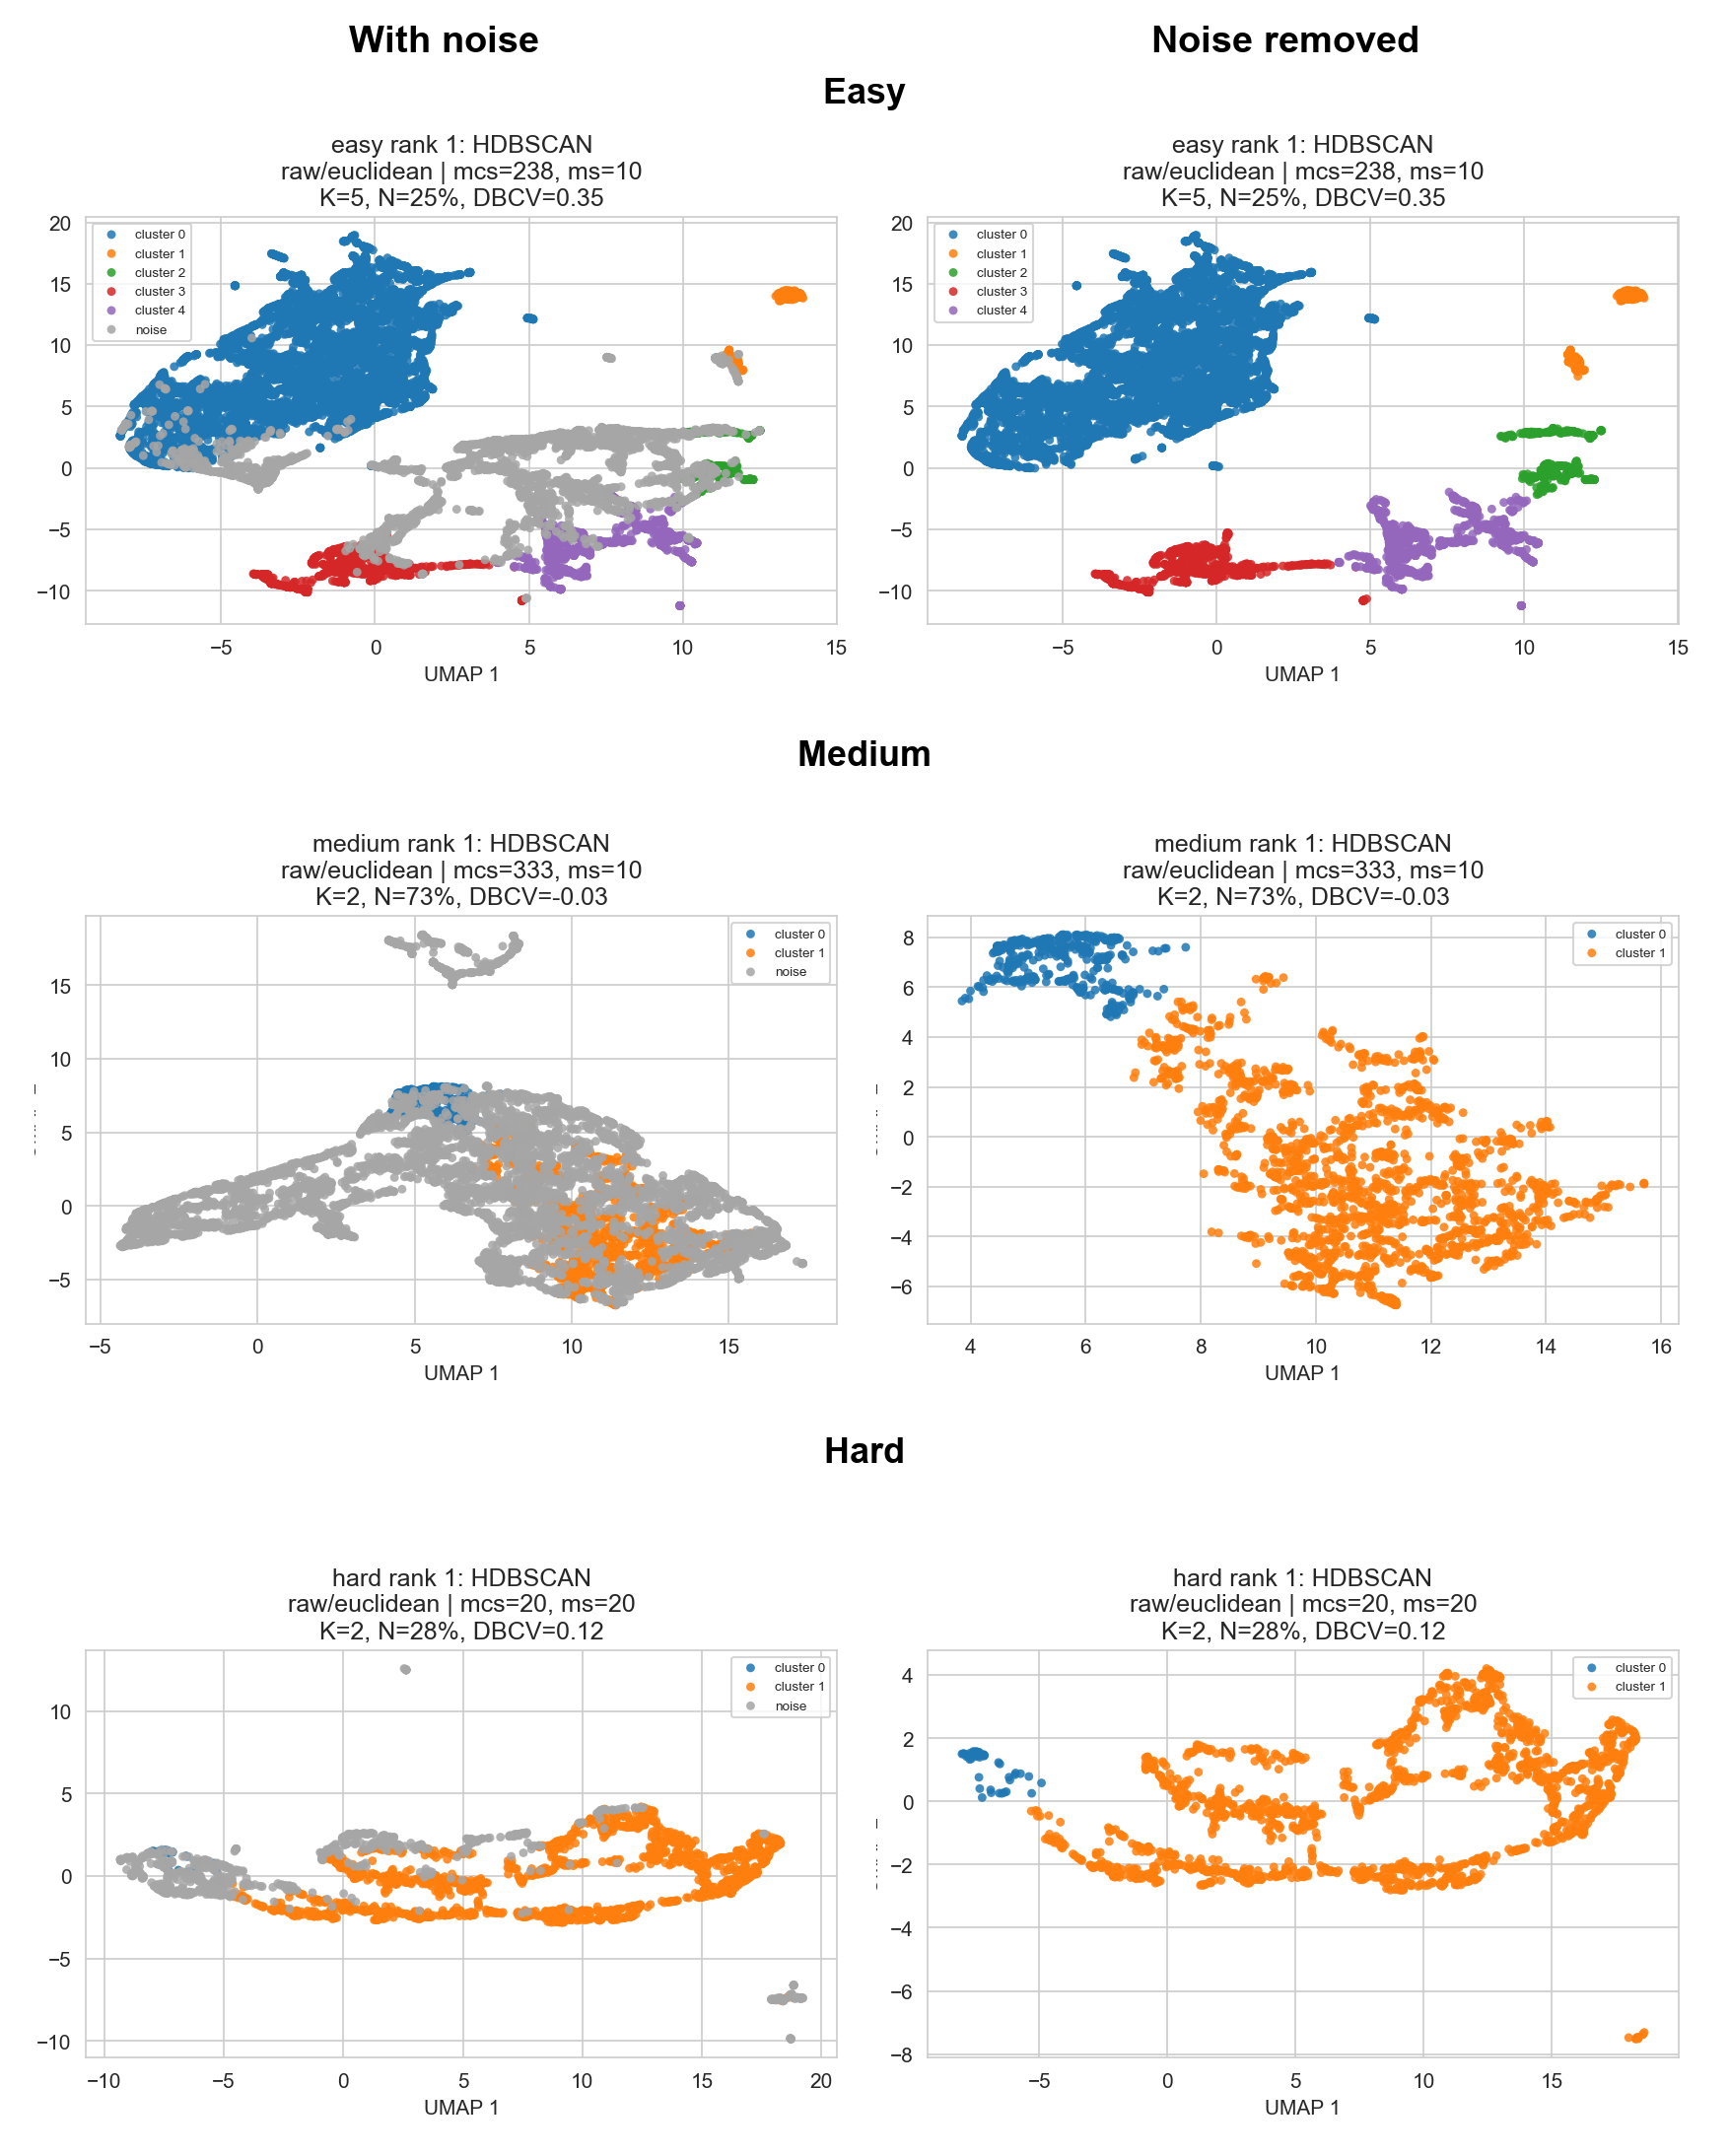
\includegraphics[width=0.86\textwidth]{figures/cluster_umap_gam_hdbscan_noise_compare.png}
  \caption{GAM--HDBSCAN additive-effect UMAP diagnostics. Rows show the easy, medium, and hard performance groups; the left column includes HDBSCAN noise points and the right column removes them.}
  \label{fig:appendix_gam_hdbscan_umaps}
\end{figure}

\subsection{DBCV Definition}
\label{app:dbcv_details}

Density-Based Clustering Validation (DBCV) evaluates whether clusters are internally dense and separated from other clusters by lower-density regions. For a cluster $C_i$, the cluster-level validity is

\begin{equation}
  V(C_i)=
  \frac{\min_{j\neq i}\mathrm{DSPC}(C_i,C_j)-\mathrm{DSC}(C_i)}
       {\max\!\left(\min_{j\neq i}\mathrm{DSPC}(C_i,C_j),\,\mathrm{DSC}(C_i)\right)}.
  \label{eq:dbcv_cluster_validity}
\end{equation}

Here $\mathrm{DSC}(C_i)$ is the density sparseness of cluster $C_i$, interpreted as the weakest internal density connection, and $\mathrm{DSPC}(C_i,C_j)$ is the density separation between clusters $C_i$ and $C_j$. The overall score averages these cluster validities by cluster size:

\begin{equation}
  \mathrm{DBCV} =
  \sum_{i=1}^{K} \frac{|C_i|}{|\mathcal{O}|}\, V(C_i).
  \label{eq:dbcv_overall}
\end{equation}

The score ranges from $-1$ to $1$. Positive values indicate dense, separated clusters; values near $0$ indicate ambiguous density structure; negative values indicate an implausible partition. Noise points have no own validity term, but they remain part of $\mathcal{O}$ in the denominator and therefore reduce the weighted support of the clustered structure.

\textcolor{red}{Note: add a formal reference for the DBCV score, e.g. Moulavi et al. (2014).}

\textcolor{red}{Note: verify the DBCV formula and interpretation against the final cited source before submission.}

\newpage

\section{Electronic appendix}
\label{el_app}

Data, code and figures are provided in electronic form.

\newpage
    
% ------------------------------------------------------------------------------
% BIBLIOGRAPHY -----------------------------------------------------------------
% ------------------------------------------------------------------------------

\RaggedRight
\bibliography{bibliography}
\bibliographystyle{dcu}
\newpage

% ------------------------------------------------------------------------------
% DECLARATION OF AUTHORSHIP-----------------------------------------------------
% ------------------------------------------------------------------------------

\Large
\noindent
\textbf{Declaration of authorship} 
\vspace{0.5cm}
\noindent
\normalsize

I hereby declare that the report submitted is my own unaided work. All direct 
or indirect sources used are acknowledged as references. I am aware that the 
Thesis in digital form can be examined for the use of unauthorized aid and in 
order to determine whether the report as a whole or parts incorporated in it may 
be deemed as plagiarism. For the comparison of my work with existing sources I 
agree that it shall be entered in a database where it shall also remain after 
examination, to enable comparison with future Theses submitted. Further rights 
of reproduction and usage, however, are not granted here. This paper was not 
previously presented to another examination board and has not been published.
\\

\vspace{1cm}
\textcolor{orange}{Location, date} \\

\vspace{3cm}

\noindent\rule{0.5\textwidth}{0.4pt} \\

\textcolor{orange}{Name}

% ------------------------------------------------------------------------------

\end{document}
